% XeLaTeX can use any Mac OS X font. See the setromanfont command below.
% Input to XeLaTeX is full Unicode, so Unicode characters can be typed directly into the source.

% The next lines tell TeXShop to typeset with xelatex, and to open and save the source with Unicode encoding.

%!TEX TS-program = xelatex
%!TEX encoding = UTF-8 Unicode

\documentclass[12pt,oneside,a4paper]{report}
\usepackage[bookmarks=true, bookmarksopen=true, colorlinks=false, linkcolor=black, driverfallback=dvipdfm, pdfstartview=FitH, hidelinks]{hyperref}	%在PDF中增加Bookmaker

\usepackage{color}
\definecolor{bisque}{rgb}{.996,.891,.755}

\usepackage[top=2.5cm,bottom=2.75cm,left=2.5cm,right=2.5cm]{geometry}   %設定頁面留白

\usepackage[boldfont,slantfont,CJKnumber,CJKspace]{xeCJK}	%xeCJK套件
\usepackage{CJKnumb}
\setmainfont{Times New Roman}								%設定英文預設字體
\setCJKmainfont{標楷體}                                      %設定中文預設字體
\setCJKsansfont{標楷體}
% \setCJKmainfont{cwTeX Q Kai Medium}                       %若標楷體無法使用之中文預設字體
% \setCJKsansfont{cwTeX Q Kai Medium}

\usepackage{eso-pic}										%插入浮水印
\usepackage{graphicx}										%插入圖片
\usepackage[bf,indentfirst,pagestyles]{titlesec}			%定義章節名稱與文字型態
\usepackage{titletoc}										%定義章節名稱
\usepackage{cite}											%bibliography package
\usepackage{tabularx}
\usepackage{longtable}										%處理長表格
\usepackage{enumitem}
\usepackage{array}
\usepackage{float}
\usepackage{fancyvrb}
\usepackage{fancyhdr}
\usepackage[above]{placeins}
\usepackage{pstricks,pst-node,pst-tree}
\usepackage{wrapfig}
\usepackage{graphicx}
\graphicspath{ {./img/} }
\usepackage{caption}
\usepackage{subcaption}
\usepackage{listings}
\usepackage{pdfpages}

%定義環境變數與巨集指令
%-------------------基本設定------------------------------------%
% 沿用 latex 的一些標點的轉換,如 en-dash 以兩個減號表示
\defaultfontfeatures{Mapping=tex-text}
\XeTeXlinebreaklocale "zh"
\XeTeXlinebreakskip = 0pt plus 1pt
%-------------------------------------------------------------%

%-------------------重新定義章節名稱格式--------------------------%
\titleformat{\chapter}[hang]{\centering\huge\bfseries}{第\CJKnumber{\thechapter}章}{1em}{}
%\renewcommand\chaptername{Chapter\hspace{.5em}\thechapter}
\renewcommand\contentsname{目錄}
\renewcommand\listfigurename{圖目錄}
\renewcommand\listtablename{表目錄}
\newcommand{\loflabel}{圖} % 定義圖目錄顯示方式
\newcommand{\lotlabel}{表} % 定義表目錄顯示方式


\titlecontents{chapter}[0pt]{}
    {第\CJKnumber{\thecontentslabel}章\quad}{}
    {\hspace{.5em}\titlerule*[10pt]{$\cdot$}\contentspage}
\titlecontents{section}[2em]{}
    {\thecontentslabel\quad}{}
    {\hspace{.5em}\titlerule*[10pt]{$\cdot$}\contentspage}
\titlecontents{subsection}[4em]{}
    {\thecontentslabel\quad}{}
    {\hspace{.5em}\titlerule*[10pt]{$\cdot$}\contentspage}

\renewcommand{\bibname}{參考文獻}            %修改參考文獻的標題名
\titlespacing{\chapter}{0pt}{*0}{*4}        %設定標題與四周的距離
\titlelabel{\thetitle\quad}				    %設定章節標題的樣式
\renewcommand{\figurename}{圖}
\renewcommand{\tablename}{表}
%-----------------------------------------------------------------%

%-------------------設定行距--------------------------------------%
\renewcommand{\baselinestretch}{2.1} % 大約等於word1.5倍行高

%設定enumerate等的item間距
\usepackage{enumitem}
\setenumerate{itemsep=-5pt}
\setitemize{itemsep=-5pt}
\setdescription{itemsep=-5pt}
%-----------------------------------------------------------------%

%-------------------定義浮水印------------------------------------%
\newcommand\WatermarkPicture{
   \put(0,0){
   \parbox[b][\paperheight]{\paperwidth}{
     \vfill
     \centering
     
\includegraphics[width=5cm,keepaspectratio]{watermark_ntut.png}%
     \vfill
     }
   }
}
%-----------------------------------------------------------------%

%------------------圖片巨集---------------------------------------%

%巨集格式
%mygraphic{圖片KeyWord}{圖片註解}{圖片路徑}
\def\myGraphic#1#2#3
{
	\begin{figure}[!htbp]
		\begin{center}
			\includegraphics[width=\textwidth]{#3}
			\caption{#2}\label{#1}
		\end{center}

	\end{figure}
}
%-----------------------------------------------------------------%

%------------------小小圖片巨集---------------------------------------%

%巨集格式
%mygraphic{圖片KeyWord}{圖片註解}{圖片路徑}
\def\myGraphicSS#1#2#3
{
	\begin{figure}[!htbp]
		\begin{center}
			\includegraphics[width=2cm]{#3}
			\caption{#2}\label{#1}
		\end{center}

	\end{figure}
}
%-----------------------------------------------------------------%

%------------------小圖片巨集---------------------------------------%

%巨集格式
%mygraphic{圖片KeyWord}{圖片註解}{圖片路徑}
\def\myGraphicS#1#2#3
{
	\begin{figure}[!htbp]
		\begin{center}
			\includegraphics[width=6cm]{#3}
			\caption{#2}\label{#1}
		\end{center}

	\end{figure}
}
%-----------------------------------------------------------------%

%------------------中圖片巨集---------------------------------------%

%巨集格式
%mygraphic{圖片KeyWord}{圖片註解}{圖片路徑}
\def\myGraphicM#1#2#3
{
	\begin{figure}[!htbp]
		\begin{center}
			\includegraphics[width=8cm]{#3}
			\caption{#2}\label{#1}
		\end{center}

	\end{figure}
}
%-----------------------------------------------------------------%

%------------------大圖片巨集---------------------------------------%

%巨集格式
%mygraphic{圖片KeyWord}{圖片註解}{圖片路徑}
\def\myGraphicB#1#2#3
{
	\begin{figure}[!htbp]
		\begin{center}
			\includegraphics[width=12cm]{#3}
			\caption{#2}\label{#1}
		\end{center}

	\end{figure}
}
%-----------------------------------------------------------------%

%------------------大大圖片巨集---------------------------------------%

%巨集格式
%mygraphic{圖片KeyWord}{圖片註解}{圖片路徑}
\def\myGraphicBB#1#2#3
{
	\begin{figure}[!htbp]
		\begin{center}
			\includegraphics[width=16cm]{#3}
			\caption{#2}\label{#1}
		\end{center}

	\end{figure}
}
%-----------------------------------------------------------------%

%------------------表格巨集---------------------------------------%
\renewcommand{\arraystretch}{1}

%巨集格式
%myTable{Table KeyWord}{Table註解}
\def\myTable#1#2
{
	\begin{table}[!htbp]
	\setlength{\abovecaptionskip}{0pt}
	\setlength{\belowcaptionskip}{10pt}
	\begin{center}
	\caption{#2}\label{#1}
}


\def\endmyTable
{
	\end{center}
	\end{table}
}

%-----------------------------------------------------------------%

%------------------修改圖與表的註解編號格式-----------------------%

\makeatletter
\long\def\@makecaption#1#2{%
  \vskip\abovecaptionskip
  \sbox\@tempboxa{{#1}\quad #2}%
  \ifdim \wd\@tempboxa >\hsize
    {#1}\quad #2\par
  \else
    \global \@minipagefalse
    \hb@xt@\hsize{\hfil\box\@tempboxa\hfil}%
  \fi
  \vskip\belowcaptionskip}
\makeatother

%-----------------------------------------------------------------%
%------------------修改Description縮排格式--------------------------%
%\makeatletter
%\renewenvironment{description}
%  {\list{}{\leftmargin\z@ \labelwidth\z@ \itemindent-\leftmargin
%   \let\makelabel\descriptionlabel}}
%  {\endlist}
%\makeatother
%-----------------------------------------------------------------%
%------------------Use Case巨集---------------------------------------%
%巨集格式
%useCase{UseCase名稱}{UseCase圖片路徑}
\def\useCase#1#2#3
{
	\subsection{#1}
	\begin{figure}[!htb]
		\begin{center}
			\includegraphics[width=\textwidth]{#2}
		\end{center}
	\end{figure}
}
% \graphicspath{{./picture/eps/}{./picture/png/}}
% \graphicspath{{.}}					%告訴Latex去這兩個目錄下找圖檔
%-----------------------------------------------------------------%
%-------------------為了方便所設定的巨集--------------------------%
\definecolor{light-gray}{gray}{0.9}
\lstset{
	basicstyle=\linespread{1.0}\ttfamily\footnotesize,
	backgroundcolor= \color{light-gray},
    rulesepcolor= \color{gray}, %程式碼塊邊框顏色
	xleftmargin = 0.7cm,
    breaklines=true,  %程式碼過長則換行
	showstringspaces=true,
    % commentstyle=\color{gray}, %註釋顏色
    frame=tlbr,    %用方框框住程式碼塊
	framesep=0.2cm,
	framerule=0pt,
}
% \setbox0 = \hbox{ttfamily}


%-----------------------------------------------------------------%


\begin{document}

\includepdf[pages={1}]{bookname.pdf}                        %封面

\AddToShipoutPicture{\WatermarkPicture}                     % 加入浮水印

\pagenumbering{roman} 										%論文篇前之頁數為羅馬數字
\chapter*{摘~~要}
\addcontentsline{toc}{chapter}{中文摘要}

%基本資訊

\noindent
論文名稱:支援多國語言的Robot Framework網頁自動化驗收測試工具的功能改善與擴充\\
頁數:XX頁\\
校所別:國立台北科技大學~資訊工程系碩士班\\
畢業時間:一百一零學年度第二學期\\
學位:碩士\\
研究生:林稟宸\\
指導教授:謝金雲、鄭有進教授\\
\hspace*{\fill}\\
\noindent
相關名詞:Robot Framework、xpath、關鍵字(Keyword)、代理關鍵字(Keyword Proxy)、i18n\\
\hspace*{\fill}\\
%
\indent
以往基於Robot Framework的網頁驗收測試,同一份測試腳本的測試對象往往只限於一種語言的網頁,
但現今的國際化社會,隨著商業模式的改變,一個網頁可能有多種語言的版本給不同國家的人使用。
為了做出類似或相同的測試目的,測試人員需要撰寫更多重複性高的測試腳本,如此一來,測試的成本便會大大增加。

根據朱峻平的論文: ”支援多國語言的Robot Framework 網頁自動化驗收測試” (i18n),
透過使用者提供的JSON格式多國語言網頁翻譯檔,建立出一份單字對應翻譯的翻譯路徑檔,
並在程式中定義翻譯的邏輯以及代理關鍵字,即可在不改動Robot Framework 測試腳本的情況下,
完成多國語言網頁自動化驗收測試。

然而,現在的i18n工具仍然存在著許多待改善之處,會造成使用上的困難。
分別是: 支援的Robot Framework原生關鍵字只有七種、翻譯邏輯只支援三種HTML屬性、
一詞多譯無法讓使用者選擇期望的翻譯、該工具尚未發佈並支援安裝。因此,本論文將針對上述幾點待改善的地方,
進行功能上的補強,希望藉此讓i18n工具在未來變得更易於使用。

										%中文摘要
\chapter*{ABSTRACT}
\addcontentsline{toc}{chapter}{ABSTRACT}

%基本資訊

\noindent
Title: Further Improvement and Extension of an Automated Web Testing Tool 
with Robot Framework to Support Internationalization\\
Pages: \\
School: National Taipei University of Technology\\
Department: Computer Science and Information Engineering\\
Time: June,2021\\
Degree: Master\\
Researcher: Bing-Chen Lin\\
Advisor: C.-Y. Hsieh and Y.C.Cheng\\
\hspace*{\fill}\\
Related terms: Robot Framework, xpath, Keyword, Keyword Proxy, I18n\\
\hspace*{\fill}\\
%
\indent
In the past, the test target of an acceptance test script with Robot Framework 
was often a  web page with single language. However, 
nowadays a web page may have multiple language versions for people 
who live in different countries. Therefore, test engineers often need to 
write test scripts which are highly repetitive, 
and the cost of testing would also increase.

According to the thesis “Internationalization Support for Automated Web Testing
with Robot Framework”(i18n) written by Chun-Ping Chu, i18n tool can build 
the mapping between words and their translations by JSON format translation 
files given by user. Besides, through the translation logic and 
keyword proxies implemented in i18n tool, we can run web tests which have 
same movements but different languages by a same test script without changing a word.

However, the i18n tool still have many flaws to be improved currently; namely, 
supporting only 7 Robot Framework native keywords, limiting to 3 HTML attributes as translate targets, 
not supporting user choices to translations of words, not supporting installation by pip.

Therefore, I will improve the flaws of the i18n tool mentioned above. 
Hoping that the i18n tool would be better and more user-friendly in the future.

										%英文摘要
\chapter*{誌~謝~}
\addcontentsline{toc}{chapter}{誌謝}

首先感謝父母對我從小到大的栽培,也感謝教授在北科的這兩年,不但教我們程式設計,
也讓我從實驗室不輕鬆卻充實的日常中收穫良多。也感謝實驗室的同學們、學弟妹兩年的陪伴。

在論文的研究過程中,感謝發哥提供了我許多寶貴的意見與討論,也特別感謝朱峻平學長,
工作之餘抽空指引我論文的研究方向,共同討論如何讓此i18n工具成為一個更好的設計。

不期望可以做出多偉大的軟體,但要做出一個有用的軟體。本論文秉持著這一精神,盡力在細節處做到最好,
不好或缺失的地方也在論文限制處如實敘述,希望透過現在的努力與之後的維護,能讓”在不改動腳本下,
實現多國語言網頁自動化驗收測試”的i18n工具,在日後成為測試者們心中的一個選項。

最後,也和自己說聲辛苦了,寫論文不像平時隨手寫一些有趣的專案那般信手拈來,要說過程中完全沒有遭遇挫折
,我相信那是騙人的。謝謝自己的堅持,才有了今天的成果,也祝自己早日交到女朋友。

程式雖然不像人一般有感情,但一旦你投入心血,它卻不會背叛你,共勉之。

											%誌謝
\newpage


\addcontentsline{toc}{chapter}{目錄}
\tableofcontents 											%引入目錄
\newpage

\addcontentsline{toc}{chapter}{表目錄}
\renewcommand{\numberline}[1]{\lotlabel~#1\hspace*{1em}}
\listoftables												%引入表目錄
\newpage

\addcontentsline{toc}{chapter}{圖目錄}
\renewcommand{\numberline}[1]{\loflabel~#1\hspace*{1em}}
\listoffigures												%引入圖目錄
\newpage													%換新頁

\pagenumbering{arabic}										%論文內文之頁數為阿拉伯數字

\chapter{緒論}

\section{研究背景與動機}
根據朱峻平的論文:「支援多國語言的Robot Framework 網頁自動化驗收測試」(i18n)\cite{i18n},透過使用者提供的JSON格式\cite{json}多國語言網頁翻譯檔,建立出一份單字對應翻譯的翻譯路徑檔,並在程式中定義翻譯的邏輯以及代理關鍵字,即可在不改動Robot Framework測試腳本的情況下,完成多國語言網頁自動化驗收測試。

然而,現在的i18n\cite{internationalization}工具仍然存在著許多待改善之處,例如: 

\begin{itemize}
\item[1.] 目前i18n工具只支援7種Robot Framework\cite{rf}原生關鍵字,如果未來測試腳本使用到其他未支援的Robot Framework原生關鍵字,便會發生錯誤。
\item[2.] 程式目前的翻譯對象僅限於網頁上的text()、normalize-space()、@title三種HTML屬性。屆時,若使用者的測試腳本是用沒有列舉出來的屬性撰寫,例如:@placeholder、@arial-label等等,便會出錯。
\item[3.] 測試腳本執行期間,若遭遇一詞多譯的情況,目前i18n工具僅於報表上列出該待翻譯詞的可能翻譯有哪些,並從中選取會使測試通過的翻譯詞當作當前翻譯;然而,使用者無法自己選擇期望的翻譯去跑測試腳本。此外,假如存在多個翻譯詞都會通過此測試(可能是因為XPath\cite{xpath}\cite{stablexpath}使用contains語法,使得畫面上要驗證的資訊只要包含於翻譯詞,測試就會通過;又或者畫面上剛好有多個元件符合翻譯後的測試腳本),翻譯過後腳本的測試對象,就會偏離了使用者原先的預期。
\\ \hspace*{\fill} \\ 
\item[4.] 目前i18n工具尚未包裝成可以讓使用者直接安裝後使用的擴充工具,停留在使用者必須將github上的專案clone下來,並且在該專案上開發測試腳本的階段。如此會造成使用者的許多不便。
\end{itemize}

有鑑於此,本論文將對現有的i18n工具進行功能的改善與擴充。

\section{研究目標}
本論文旨在改善i18n工具上述提及的四項缺陷,希望透過以下努力可以讓此I18n工具在未來執行多國語言網頁自動化驗收測試\cite{se}\cite{testduo}時,更易於使用。

實作的目標分別列舉如下:
\begin{itemize}
\item[1.] 擴充完剩下的Robot Framework原生關鍵字代理,使得所有常用原生關鍵字的參數部分都能正確的被翻譯。
\item[2.] 撰寫出一套新的XPath翻譯邏輯,支援除了@title、normalize-space()、text()以外,其他HTML屬性的翻譯檢查。
\item[3.] 執行完含有一詞多譯的測試腳本後,如果測試通過,便開啟一個圖形化介面,記錄了執行翻譯時當下關鍵字的參數組合,並顯示所有可能的翻譯詞,讓使用者可以從中去選擇,並產生一個設定檔。之後再次執行測試腳本時,i18n工具便會根據設定檔的內容去選擇適當的翻譯詞,同時消除報表上的warning提示。 
\item[4.] 將i18n工具包裝成為可以pip\cite{PIP} install 的library。
\end{itemize}

\section{論文組織架構}
本論文分為五章,第一章介紹研究背景與動機,以及期望達成的研究目標。第二章介紹本論文相關的背景知識。第三章探討本論文的研究方法與實作,詳述擴充代理關鍵字的流程、改善翻譯邏輯的完整思路,以及如何藉由圖形化使用者介面去改善i18n工具目前遇到一詞多譯時的處理方法。第四章展示實際的測試案例,呈現做了上述改動後,使用者執行多國語言網頁自動化驗收測試時,會得到什麼結果,並可自行與第一版i18n工具\cite{i18n}做比較。第五章則是結論以及未來展望,概述本論文的成果以及尚且存在的使用限制和待改善之處。
\chapter{背景知識}

\section{國際化}
國際化(Internationalization)\cite{internationalization},簡寫為i18n,其中18代表i和n之間的18個英文字母。國際化是開發軟體時,將軟體本身和特定語言、地區脫鉤的一個過程,除了可以滿足不同的地區、文化的大眾需求,移植軟體到不同的語言環境時,也不須改變內部程式的實作。

\section{自動化驗收測試}
驗收測試(Acceptance Testing)\cite{se},是一種站在使用者的立場,去檢驗一個真實存在的系統,是否滿足使用者需求與預期的測試方法。

而透過撰寫自動化測試腳本\cite{AT},如今我們可以執行更符合成本,且更加精確的自動化驗收測試。改善了過往手動執行驗收測試時,存在的人為操作誤差、系統問題無法即時呈現、成本較高等問題。
\section{Robot Framework}
Robot Framework\cite{rf}\cite{rfguide}是一個開源的框架語言,可以用來執行自動化驗收測試或機器人自動化,核心框架是由Python\cite{python}編寫而成,測試者可以使用Python或Java擴充其函式庫。其特色是擁有簡單的語法,以及容易理解的原生關鍵字(Keyword),測試者可以視需求使用並包裝成更接近自然語言的關鍵字。

\subsection{Robot Framework測試腳本}
一個Robot Framework 的測試腳本基本上由三個區塊構成,分別是:
\begin{itemize}
    \item[1.]Settings: 包含了使用到的library與resource file,也可以將Test Setup(測試腳本執行前要做的動作)、Test Teardown(測試腳本執行後要做的動作)定義於此。
    \item[2.]Test Cases: 在此測試者可以為各項想要驗證的使用者需求,撰寫核心的測試腳本
    \item[3.]Keywords: 如果測試腳本使用並非Robot Framework的原生關鍵字,或未被定義於其他resource file中,測試者可以在此處撰寫出新的關鍵字去達到測試目的。
\end{itemize}

\subsection{Robot Framework測試報表}
在測試腳本運行結束後,Robot Framework會產生出一份測試報表,記錄了整體的執行狀況,包含測試通過或失敗、腳本執行時間,並透過可展開的階層式圖表,方便測試者去追蹤到當前出現問題的關鍵字,進而修復錯誤。

\section{XPath}
XPath\cite{xpath},全名為 XML Path Language,可以用來定位XML檔案中某節點所處在的位置。在使用Robot Framework撰寫的網頁自動化驗收測試中,我們便時常需要藉助XPath,去找到並確定畫面上某元件的位置,以對其狀態進行測試。

\section{第一版i18n的系統架構與運作原理}
\begin{figure}[H]
    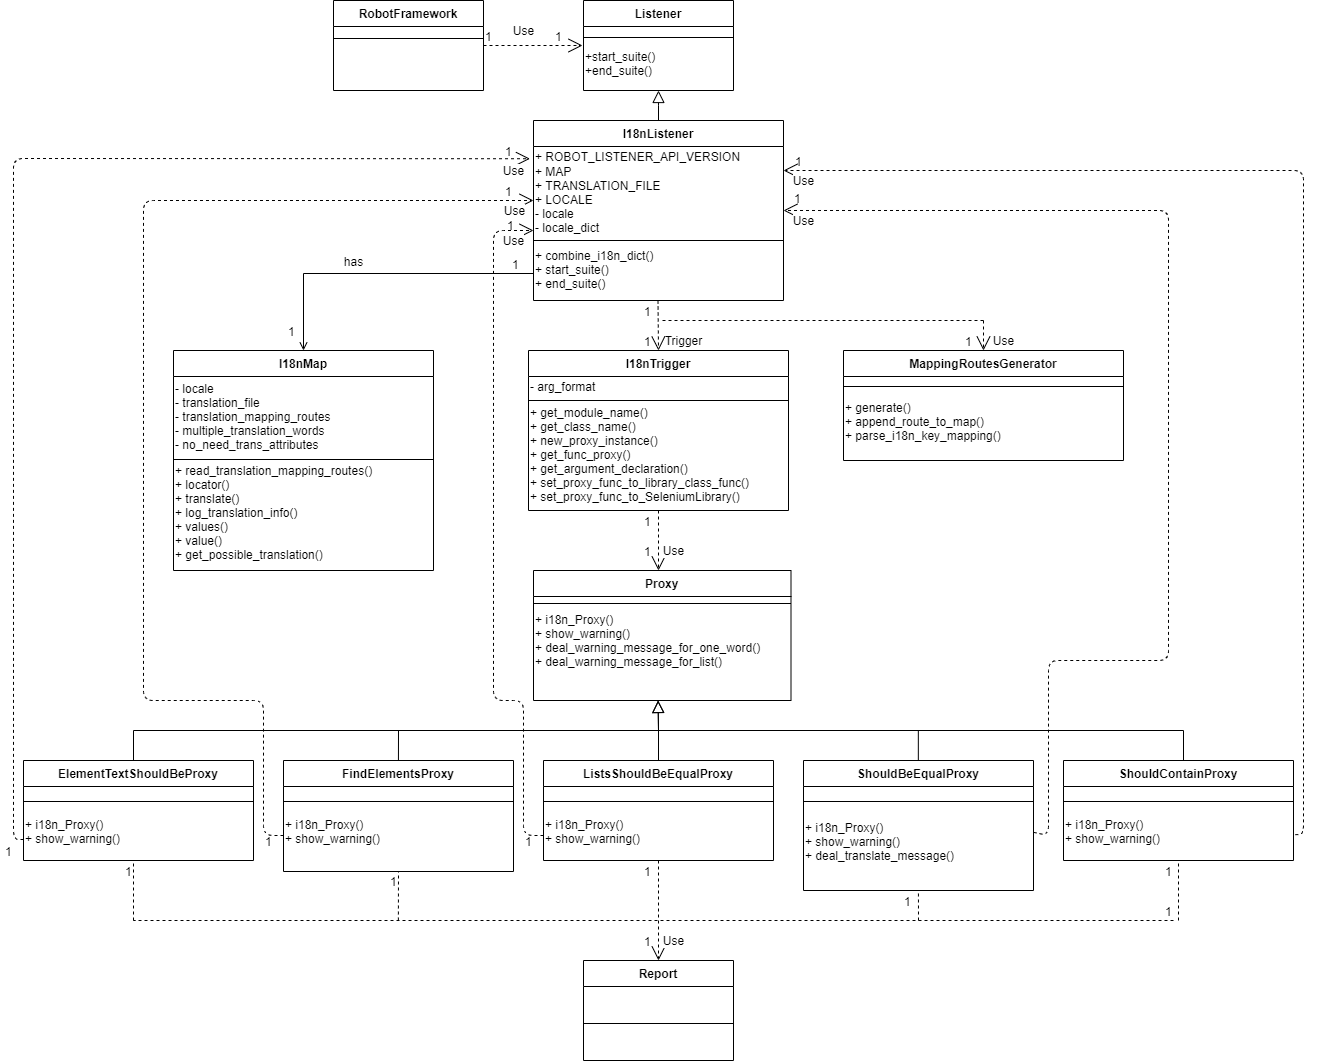
\includegraphics[width= 1.1\textwidth]{../UML/i18n class diagram-第一版i18n class diagram.png}
    \caption{第一版i18n的系統類別圖}
    \label{1stI18nClassDiagram}
\end{figure}
第一版i18n的系統類別圖(如圖~\ref{1stI18nClassDiagram}),包含了3個 Robot Framework原生類別: RobotFramework、Listener、和Report;第一版i18n所設計的5個系統類別 :I18nListener、MappingRoutesGenerator、I18nMap、I18nTrigger、Proxy,以及5個實作自Proxy\cite{proxy}類別的代理關鍵字類別: ShouldContainProxy、ElementTextShouldBeProxy、FindElementProxy、ListsShouldBeEqualProxy、ShouldBeEqualProxy。\cite{i18n}

I18nListener類別實作Listener類別,負責程式開始與結束時執行start\_suite()和end\_suite()的內容,並對MappingRoutesGenerator、I18nMap、I18nTrigger三個類別進行初始化的動作。I18nMap類別負責處理各個代理關鍵字類別透過I18nListener類別的呼叫,並將待翻譯詞做翻譯後回傳。I18nTrigger類別透過new\_proxy\_instance()函式建立各個代理關鍵字類別的實例;並使用set\_proxy\_func\_to\_library\_class\_func()、set\_proxy\_func\_to\_SeleniumLibrary()兩函式,將代理關鍵字類別的實作包裝於Robot Framework原生關鍵字之外,使每次呼叫關鍵字時,必先執行代理關鍵字的實作。MappingRoutesGenerator類別負責以英文JSON翻譯檔為基準,產生出翻譯路徑檔,讓測試腳本運行在其他語言環境下,可以根據此路徑,在所屬語言的JSON翻譯檔下找到正確的翻譯。Proxy類別提供了一個介面,讓實作Proxy類別的代理關鍵字類別可以根據各自的需要,去擴充內部的實作;其中,i18n\_Proxy()函式提供各代理關鍵字類別撰寫核心的功能。

\begin{figure}[H]
    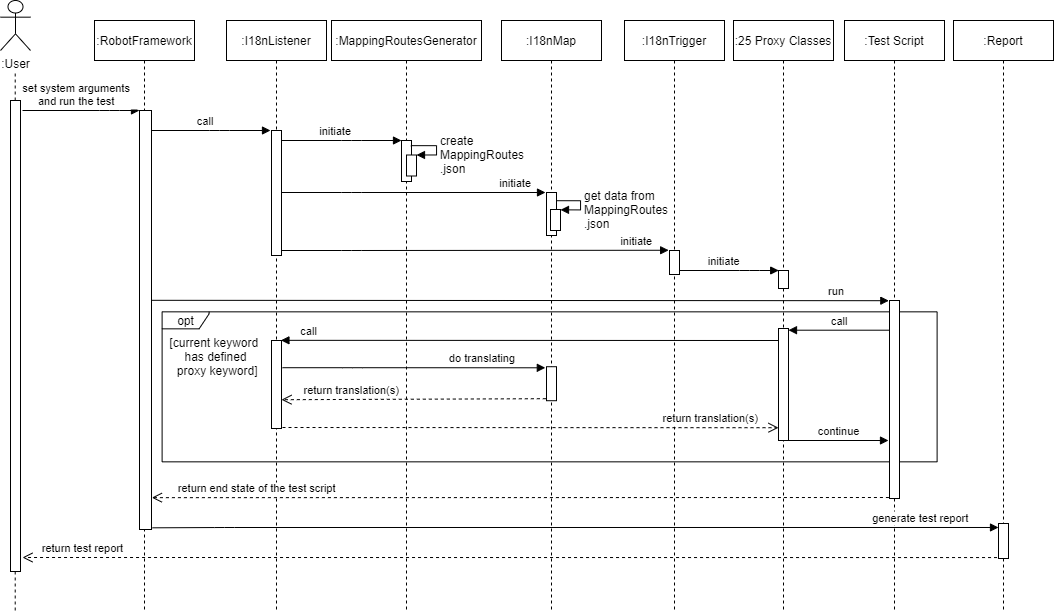
\includegraphics[width= 1.1\textwidth]{../UML/i18n sequence diagram-第一版i18n系統流程.png}
    \caption{第一版i18n的系統流程Sequence Diagram}
    \label{1stI18nSequenceDiagram}
\end{figure}
系統流程的部分(如圖~\ref{1stI18nSequenceDiagram}),在使用i18n工具執行測試腳本前,使用者必須於Red編輯器\cite{red}中的Additional Robot Framework arguments設定系統參數為-d out –L debug -–listener i18n/listeners/I18nListener.py:zh-TW,zh-TW代表當前語言為繁體中文-台灣(如圖~\ref{rfSysArgsSetting})。

\begin{figure}[H]
    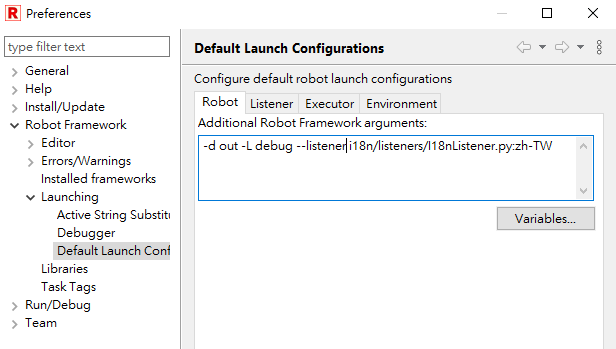
\includegraphics[width= 1.1\textwidth]{../論文截圖/3-1-3-1 設定系統參數.png}
    \caption{Robot Framework系統參數設定}
    \label{rfSysArgsSetting}
\end{figure}
測試執行時,系統會先去呼叫I18nListener類別並執行其實作。之後初始化MappingRoutesGenerator類別,藉由讀取由使用者自行提供的JSON格式翻譯檔(如圖~\ref{英文的JSON格式翻譯檔示例}),建立出一份由「待翻譯詞」和「Key階層」構成的翻譯路徑檔(如圖~\ref{翻譯路徑檔});例如待翻譯詞‘Support’,有兩種Key階層的路徑: "['SUPPORT']" 和 "['SUB\_BAR']['BLUE\_TITLE']['MICROSOFT\_SUPPORT']",代表‘Support’在多國語言網頁中,會在不同情境下被翻譯成兩種不同的詞彙。接著系統會依序初始化I18nMap、I18nTrigger,以及所有代理關鍵字類別。

當執行完上述工作後,測試腳本才會正式開始執行;每當腳本運行到一個有定義代理的關鍵字,系統就會去呼叫對應的代理關鍵字物件,並執行翻譯邏輯。最後,當測試腳本執行結束,系統則會將一詞多譯的warning資訊顯示在報表上。

\begin{figure}[H]
    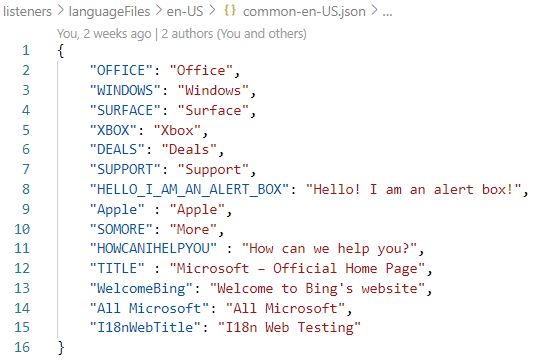
\includegraphics[width= 1.1\textwidth]{../論文截圖/3-1-3-2 JSON格式翻譯檔.png}
    \caption{英文的JSON格式翻譯檔示例}
    \label{英文的JSON格式翻譯檔示例}
\end{figure}

\begin{figure}[H]
    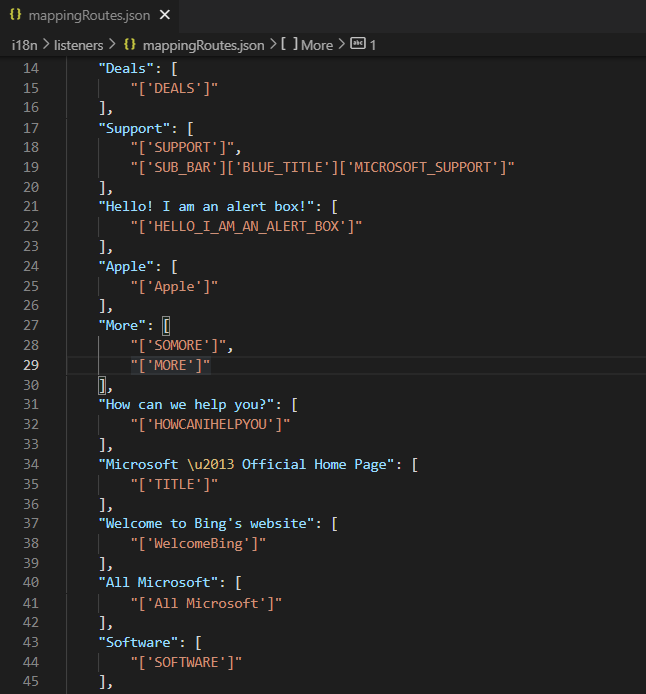
\includegraphics[width= 1.1\textwidth]{../論文截圖/3-1-3-3 翻譯路徑檔.png}
    \caption{翻譯路徑檔部分示例}
    \label{翻譯路徑檔}
\end{figure}

\chapter{研究方法與實作}
本章將詳述如何針對i18n工具現存的四項問題,進行思考與改善,並點出與朱峻平的論文「支援多國語言的Robot Framework網頁自動化驗收測試」(第一版i18n工具)的不同之處。

%3.1
\section{系統擴充}
新版i18n系統類別圖(如圖~\ref{新版i18n系統類別圖}),沿用第一版i18n工具的架構(如圖~\ref{1stI18nClassDiagram}),經過部分實作的改善,並且新增了一個用於顯示一詞多譯選項的圖形化使用者介面類別(UI),以及20種代理關鍵字的類別。(新增的類別在圖中以紅色方框標示)

\begin{figure}[H]
\flushleft
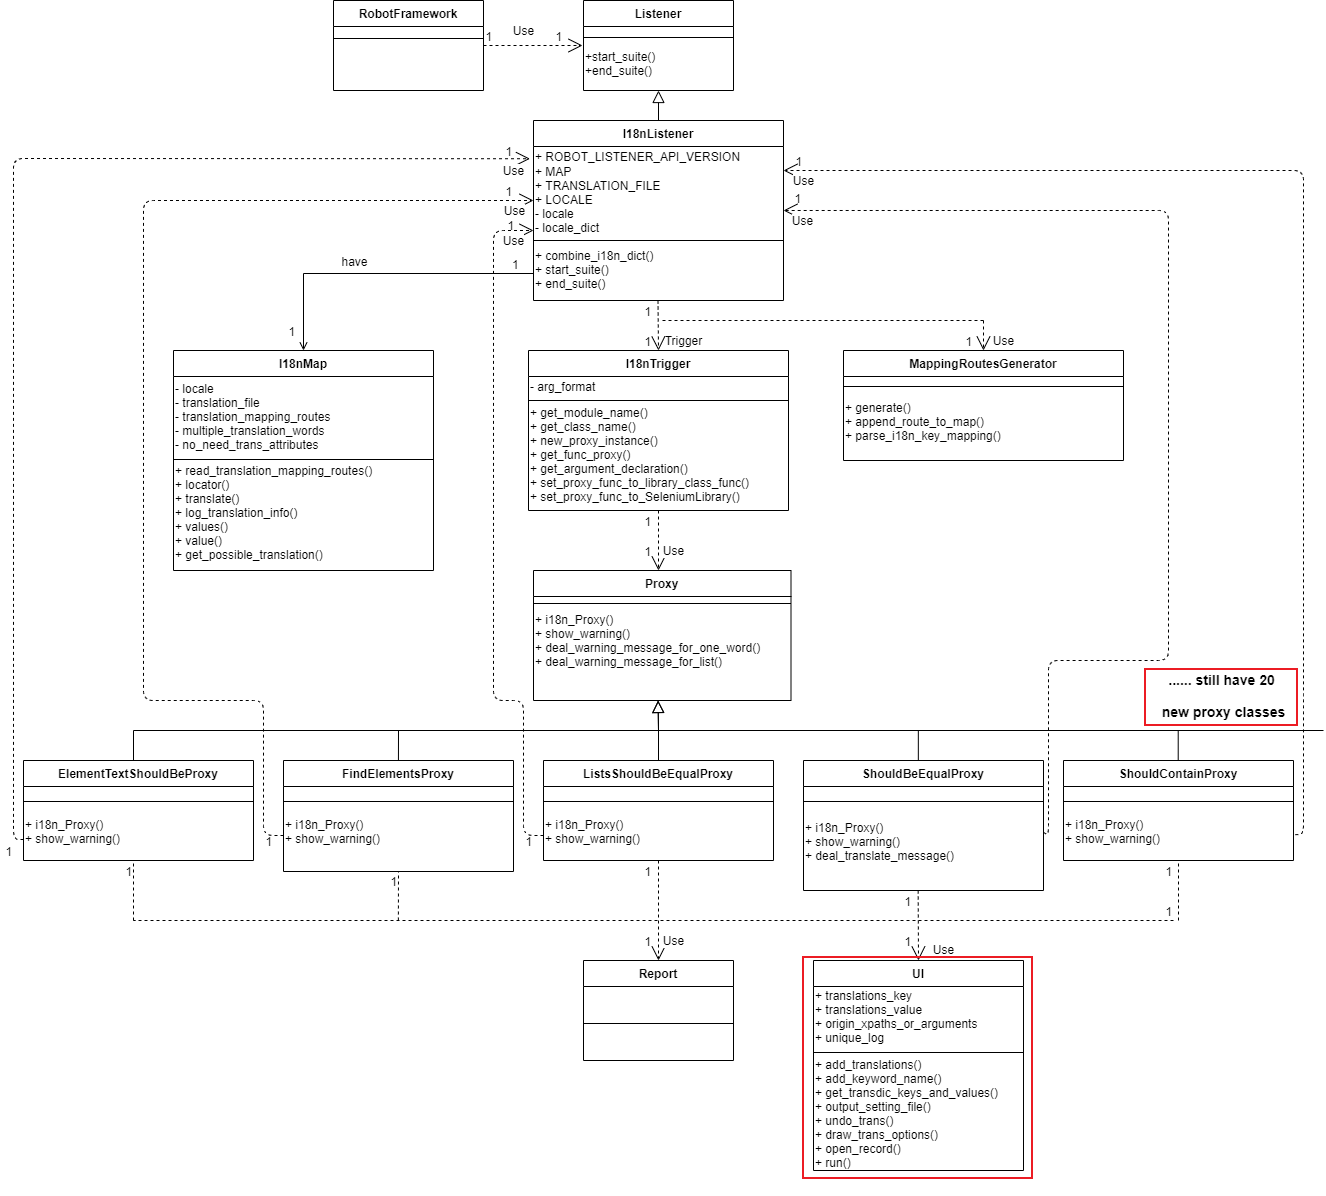
\includegraphics[width= 180mm]{../UML/i18n class diagram-i18n class diagram.png}
\caption{新版i18n系統類別圖}
\label{新版i18n系統類別圖}
\end{figure}

本論文新增的UI類別會在程式執行期間,記錄下遭遇到一詞多譯的詞語以及其翻譯。在程式執行後,產生一詞多譯的UI;使用者選擇並提交希望的翻譯後,便會產生一個系統設定檔記錄翻譯選擇。

而其他20種新增的代理關鍵字類別(如表~\ref{本論文新增的20種代理關鍵字類別}),皆實作父類別Proxy,負責代理各自對應之原生關鍵字的參數部分翻譯,並將翻譯好的參數部分回傳給對應的原生關鍵字。

\hspace*{\fill} \\

\begin{table}[H]
    \centering
        \begin{tabular}{|l|l|}
        \hline
        \multicolumn{2}{|c|}{新增的代理關鍵字類别} \\ \hline
        1. AlertShouldBePresentProxy & 11. ListShouldNotContainDuplicatesProxy\\ 
        2. CountValuesInListProxy & 12. RemoveFromDictionaryProxy\\ 
        3. DictionariesShouldBeEqualProxy & 13. RemoveValuesFromListProxy\\
        4. DictionaryShouldContainItemProxy & 14. SelectFromListByLabelProxy\\
        5. DictionaryShouldContainKeyProxy & 15. SelectFromListByValueProxy\\
        6. DictionaryShouldContainValueProxy & 16. TableCellShouldContainProxy\\
        7. GetMatchCountProxy & 17. TableColumnShouldContainProxy\\
        8. ListSelectionShouldBeProxy & 18. TableRowShouldContainProxy\\
        9. ListShouldContainSubListProxy & 19. TableShouldContainProxy\\
        10. ListShouldContainValueProxy & 20. TitleShouldBeProxy\\   
        \hline
        \end{tabular}
    \caption{本論文新增的20種代理關鍵字類別}
    \label{本論文新增的20種代理關鍵字類別}
\end{table}

系統執行流程相較於第一版i18n改動較大的部份,是在測試腳本結束後;除了將一詞多譯的warning資訊顯示在報表上外,若是遭遇過一詞多譯,便會跳出一詞多譯的UI(詳見3-4節),記錄了執行翻譯當下關鍵字的參數組合,並顯示所有可能的翻譯詞,讓使用者可以從中去選擇並產生一個設定檔。之後再次執行測試腳本時,系統便會根據設定檔的內容去選擇適當的翻譯詞,同時消除報表上的warning提示資訊。

\hspace*{\fill} \\
\\ \hspace*{\fill} \\

%3.2
\section{擴充與修改代理關鍵字實作}
第一版i18n工具只支援7種Robot Framework原生關鍵字(如表~\ref{第一版i18n已提供的原生關鍵字})\cite{i18n}。尚有31種參數部分需要翻譯的原生關鍵字,未提供支援。如果測試腳本使用到這些未支援的原生關鍵字去執行多國語言網頁測試,則會導致出錯。因此,本論文的解法是擴充完目前Robot Framework版本剩下的代理關鍵字,使得有翻譯需求的原生關鍵字,其參數部分都能正確的被翻譯。

\renewcommand\arraystretch{0.8}
\begin{table}[H]
    \centering
    \setlength{\tabcolsep}{10mm}{
        \begin{tabular}{|l|}
        \hline
        第一版i18n已提供代理的關鍵字 \\
        \hline
        1. find\_element \\
        2. element\_text\_should\_be \\
        3. lists\_should\_be\_equal\\
        4. should\_be\_equal\\
        5. should\_not\_be\_equal\\
        6. should\_contain\\
        7. should\_not\_contain\\       
        \hline
        \end{tabular}}
    \caption{第一版i18n已提供代理的Robot Framework原生關鍵字}
    \label{第一版i18n已提供的原生關鍵字}
\end{table}

且又因為先前的i18n工具分別在Robot Framework版本3.0.4、SeleniumLibrary版本3.1.1下開發,而現在的Robot Framework版本已更新到3.2.2,SeleniumLibrary版本則更新到4.5.0,導致原先需要被支援的31種原生關鍵字,有兩種已被淘汰:
input\_text\_into\_prompt、xpath\_should\_match\_x\_times。因此,還有29種原生關鍵字需要提供代理(如表~\ref{新版i18n將擴充代理的Robot Framework原生關鍵字})。(‘*’標示為因版本更新導致被淘汰的原生關鍵字)

\begin{table}[H]
    \centering 
    \setlength{\tabcolsep}{5mm}{
        \begin{tabular}{|l|l|}
        \hline
        \multicolumn{2}{|c|}{待擴充的代理關鍵字}\\ \hline
        Collections Libaray (3.2.2) & SeleniumLibrary (4.5.0) \\ \hline
        1. count\_values\_in\_list & 1. alert\_should\_be\_present \\
        2. dictionaries\_should\_be\_equal & 2. input\_text\_into\_alert \\
        3. dictionary\_should\_contain\_item & 3. *input\_text\_into\_prompt\\    
        4. dictionary\_should\_contain\_sub\_dictionary & 4. *xpath\_should\_match\_x\_times\\    
        5. dictionary\_should\_contain\_key & 5. list\_selection\_should\_be\\    
        6. dictionary\_should\_not\_contain\_key & 6. select\_from\_list\_by\_label\\    
        7. dictionary\_should\_contain\_value & 7. unselect\_from\_list\_by\_label\\    
        8. dictionary\_should\_not\_contain\_value & 8. select\_from\_list\_by\_value\\    
        9. list\_should\_contain\_sub\_list & 9. unselect\_from\_list\_by\_value\\    
        10. list\_should\_contain\_value & 10. title\_should\_be\\    
        11. list\_should\_not\_contain\_value & 11. table\_should\_contain\\    
        12. list\_should\_not\_contain\_duplicates & 12. table\_header\_should\_contain\\    
        13. remove\_from\_dictionary & 13. table\_footer\_should\_contain\\    
        14. remove\_values\_from\_list & 14. table\_cell\_should\_contain\\    
        15. get\_match\_count & 15. table\_column\_should\_contain\\
        & 16. table\_column\_should\_contain\\
        \hline
        \end{tabular}}
    \caption{新版i18n將擴充代理的Robot Framework原生關鍵字}
    \label{新版i18n將擴充代理的Robot Framework原生關鍵字}
\end{table}
以下將以 FindElementsProxy的Flow Chart為例,詳述現今配合新增的一詞多譯UI下,本論文是如何完成代理關鍵字的擴充和修改。(沿用第一版i18n的部分會以‘*’號標註)

\begin{figure}[H]
    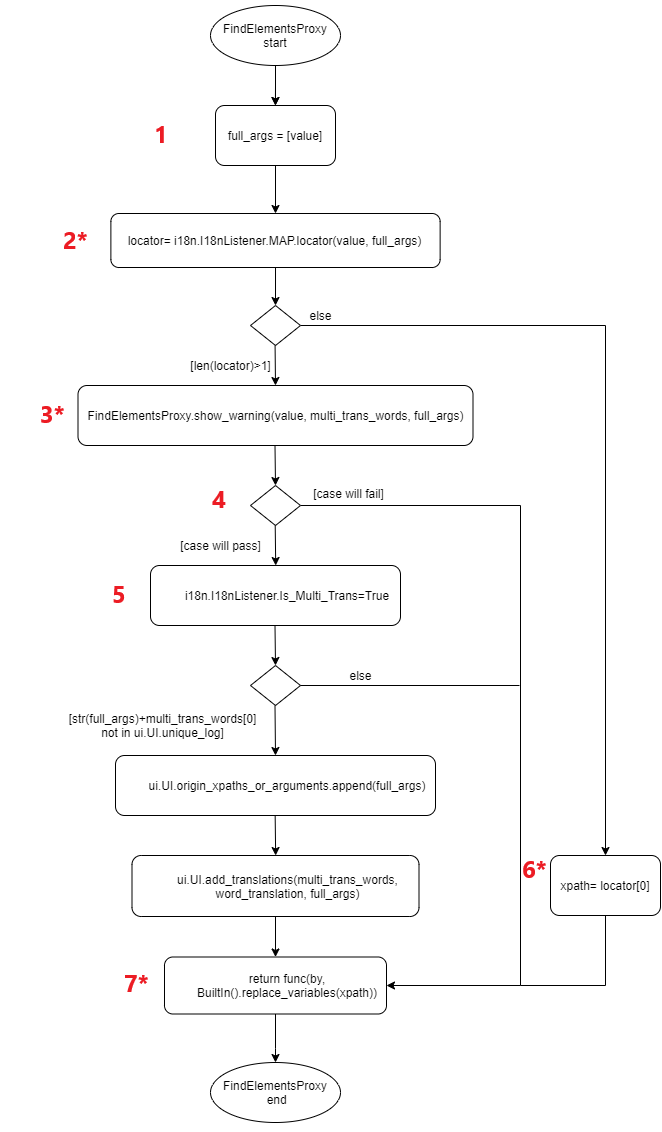
\includegraphics[width= .85\textwidth]{../UML/i18n flow chart-FindElementsProxy.png}
    \caption{FindElementsProxy的Flow Chart}
    \label{FindElementsProxy的Flow Chart}
\end{figure}

由圖~\ref{FindElementsProxy的Flow Chart} FindElementProxy的Flow Chart可以得知,在新的i18n版本下,擴充一個新的代理關鍵字必須遵從著以下步驟:(以下編號可對應到Flow Chart的數字)
\begin{itemize}
\item[1 .]創出該次關鍵字呼叫的參數紀錄變數,full\_args。此變數之後會成為判斷當下待翻譯詞是否「已被使用者選擇翻譯」的依據。並於測試腳本結束後,顯示於一詞多譯UI上,最後隨著使用者的選擇一併存入設定檔內。

\item[2*.]執行翻譯。如:
\begin{lstlisting}[language={python}]
locator = i18n.I18nListener.MAP.locator(value,full_args)
\end{lstlisting}
透過i18nListener類別的MAP變數(其內裝著i18nMap類別的初始化資訊),去呼叫i18nMap類別的locator函式,對待翻譯詞value執行翻譯,且必須代入full\_args以實現1.的內容。

\item[3*.]若判定此代理關鍵字遭遇一詞多譯,則產生warning資訊於報表上,如:
\begin{lstlisting}[language={python}]
FindElementsProxy.show_warning(value,multi_trans_words,full_args)
\end{lstlisting}

\item[4 .]之後判斷此一詞多譯情況,最後會使測試通過或是失敗,如:
\begin{lstlisting}[language={python}]
is_actual = BuiltIn().run_keyword_and_return_status('Get WebElement', translation_locator)
if is_actual:
\end{lstlisting}

\item[5 .]若測試會通過,則對預計開啟的UI做一些資料的準備,如:
\begin{lstlisting}[language={python}]
i18n.I18nListener.Is_Multi_Trans=True
if str(full_args)+multiple_translation_words[0] not in ui.UI.unique_log
ui.UI.origin_xpaths_or_arguments.append(full_args)
ui.UI.add_trans_info(self, multiple_translation_words, word_translation, full_args, func.__name__)
\end{lstlisting}
先設定再測試結束後,需要開啟一詞多譯UI。若該「參數+翻譯詞」組合尚未被翻譯過,則記錄下該次翻譯的參數部分和翻譯資訊。

\item[6*.]若此次代理關鍵字沒有遭遇一詞多譯,則如:
\begin{lstlisting}[language={python}]
xpath = locator[0]
\end{lstlisting}
將第一筆翻譯同時也是唯一一筆翻譯指派給之後要回傳的xpath。

\item[7*.]將翻譯好的參數部分回傳給Robot Framework原生關鍵字,如:
\begin{lstlisting}[language={python}]
return func(self, by, BuiltIn().replace_variables(xpath))
\end{lstlisting}
\end{itemize}

其他未能一一介紹的代理關鍵字,儘管彼此間實作仍然存在著差異,但都是遵循著以上的架構去設計。


\hspace*{\fill} \\
\\ \hspace*{\fill} \\
\\ \hspace*{\fill} \\
\\ \hspace*{\fill} \\
\\ \hspace*{\fill} \\
\\ \hspace*{\fill} \\
\\ \hspace*{\fill} \\
\\ \hspace*{\fill} \\
%3.3
\section{改善XPath翻譯邏輯使其能應對各種HTML屬性}
在第一版i18n的翻譯邏輯中,若一個XPath內部存在多種HTML屬性,i18n工具使用了列舉法(如圖~\ref{以列舉法定義要被翻譯的HTML屬性}),僅提供了@title、text()、normalize-space()三種屬性的翻譯規則。屆時,若測試腳本的XPath是用沒有列舉出來的屬性撰寫,但卻有翻譯的需求,例如:@placeholder、@arial-label等等,則會導致測試出錯。

\begin{figure}[H]
\begin{lstlisting}[language={python}]
default_rule = {
'((text|normalize-space)\((text\(\))?\) ?= ?(\'|\")(([0-9a-zA-Z.?&()]| )+)(\'|\"))': 4,
'((text|normalize-space)\((text\(\))?\)\, ?(\'|\")(([0-9a-zA-Z.?&()]| )+)(\'|\"))': 4,
'((@title) ?= ?(\'|\")(([0-9a-zA-Z.?&()]| )+)(\'|\"))' : 3,
'((@title), ?(\'|\")(([0-9a-zA-Z.?&()]| )+)(\'|\"))' : 3
}
\end{lstlisting}
\caption{以列舉法定義要被翻譯的HTML屬性}
\label{以列舉法定義要被翻譯的HTML屬性}
\end{figure}

為了解決以上問題,本論文最後決定採用「負面表列法」,將確定不會執行翻譯的HTML屬性在程式中用list的方式儲存。若XPath中的HTML屬性不在該list中,則都去執行翻譯檢查。

此種作法相較於把所有HTML屬性都執行翻譯檢查,顧及到了系統執行效能,來的更加省時。相較於設計一個複雜邏輯,來訓練系統自行判斷當前HTML屬性是否要翻譯,在實作上則更為簡單,且把翻譯的決定權交給了測試者,而非全部靠系統。相較於第一版i18n,把翻譯規則用列舉法固定,此作法則更能顧及到未來測試腳本的不確定性,因為我們無法預期使用者會用怎麼樣的方式去編寫XPath。

以下將以新版i18n XPath翻譯邏輯的Sequence Diagram為例(如圖~\ref{新版i18n XPath翻譯邏輯的Sequence Diagram}),輔以部分程式碼,詳述系統是如何根據當下情況,產生一套新的翻譯邏輯,以解決先前某些HTML屬性無法被翻譯的問題。

\begin{figure}[H]
    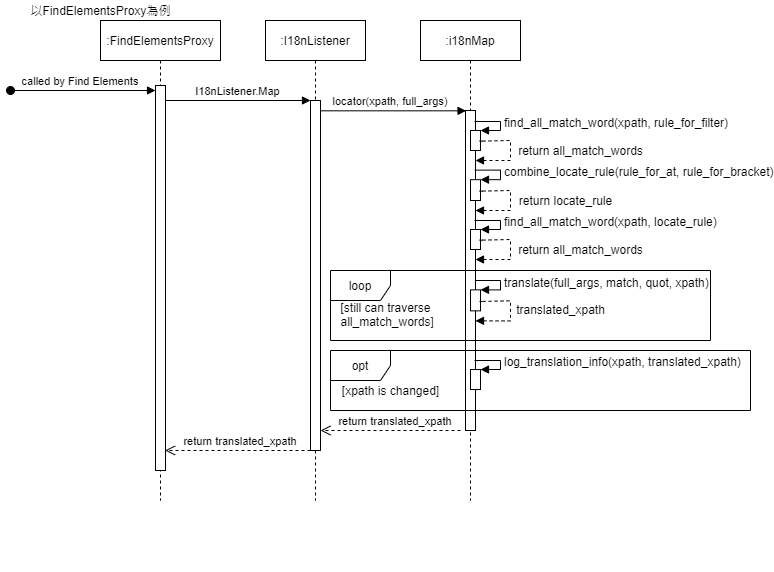
\includegraphics[width= 1.1\textwidth]{../UML/i18n sequence diagram-xpath翻譯邏輯.png}
    \caption{新版i18n XPath翻譯邏輯的Sequence Diagram}
    \label{新版i18n XPath翻譯邏輯的Sequence Diagram}
\end{figure}

首先,被呼叫後,FindElementsProxy透過I18nListener類別,呼叫I18nMap類別的locator()函式執行XPath的翻譯。之後,I18nMap先定義一個內含HTML屬性特徵的rule\_for\_filter變數,如:
\begin{lstlisting}[language={python}]
rule_for_filter = {
    "(@[a-z-]*)":"@",
    "([a-z-]*\(\))":"()"
}
\end{lstlisting}
隨後呼叫find\_all\_match\_word()函式,來過濾出XPath中包含的所有屬性。

接著,先判斷這些屬性是否包含在「不需被翻譯屬性」的list中。如:
\begin{lstlisting}[language={python}]
for rule, matches in all_match_attributes.items():
    for match in matches:
        if match not in self.no_need_trans_attirbutes:
\end{lstlisting}
若不包含其中,則根據屬性含有 ‘@’ 或 ‘()’,分別分配給rule\_for\_at和rule\_for\_bracket變數,並呼叫combine\_locate\_rule()函式,得到一套新的翻譯邏輯,locate\_rule。

之後,再次呼叫find\_all\_match\_word()函式,得到所有符合新翻譯邏輯的HTML屬性,all\_match\_words。並利用迴圈遍歷all\_match\_words中的屬性,執行translate()函式,進行翻譯檢查。
	
接著,判斷經過翻譯後,原先的xpath是否發生變化;例如xpath從原本的 //*[text()=‘Software'],變成了翻譯後的//*[text()=‘軟體']。若xpath改變,則執行log\_translation\_info()函式,將翻譯資訊顯示於測試報表上。

最後,將翻譯後的translated\_xpath,回傳給FindElementsProxy類別,完成一次XPath的翻譯。

\hspace*{\fill} \\
\\ \hspace*{\fill} \\
\\ \hspace*{\fill} \\
\\ \hspace*{\fill} \\
\\ \hspace*{\fill} \\
\\ \hspace*{\fill} \\
\\ \hspace*{\fill} \\
%3.4
\section{提供圖形化使用者介面解決一詞多譯的問題}
先前遇到一詞多譯問題時,第一版i18n工具提供了warning資訊於測試結束後的報表上,此作法確實提醒了使用者該腳本存在著一詞多譯問題,且也顯示出目前系統採用的翻譯詞,這是好的部分,本論文將繼續沿用。此翻譯邏輯是站在一個「最大化讓測試腳本通過」的立場,當遭遇一詞多譯時,系統會將所有的翻譯都執行看看,直到一包可能的翻譯中,出現了一個會使測試通過的翻譯,則算測試通過,並將該翻譯詞呈現於報表上。

然而,以上作法卻存在著一個缺陷,即是「使用者無法自由的選擇真正想要的翻譯詞」去執行腳本測試,而把決定全權授予系統。並有機會產生以下兩點問題:
\begin{itemize}
\item[1.]假如存在「多個翻譯都會使測試通過」,翻譯過後的腳本測試對象,就有機會偏離使用者原先的預期。其原因可能是XPath使用contains撰寫,使得翻譯只要包含特定詞即會讓測試通過。如: 翻譯過後的XPath為//*[@id= ‘supHomeAndLandingPageHeaderContainer]//*[contains(@text, ‘支援’)],而畫面上待驗證的元件顯示的詞是「支援服務」,測試會通過,但遺憾的是使用者預期‘Support’在此處應該要被翻譯為「支援服務」。
 
\hspace{5mm} 又或是畫面上同時存在含有不同翻譯的元件,且滿足測試腳本的XPath,而導致測試通過。如: 畫面上兩個元件,分別顯示「支援」與「支援服務」;原本使用者預期要驗證的是畫面上存在「支援服務」字樣,但因為‘Support’先被系統檢查的翻譯為「支援」,導致翻譯後的XPath //*[@text= ‘支援’]率先通過了測試,而不會再去檢驗後續的翻譯。 
\item[2.]假如此測試腳本原先就會發生錯誤,經過翻譯後的XPath卻因為碰巧滿足畫面上的某個元件,而導致測試通過。在此特殊情形下,翻譯過後的測試對象,則更明顯的偏離了使用者原先的預期,且也改變了測試結果。如: 原腳本要驗證 //*[@text='Service'],測試會失敗,但經過翻譯後XPath變成//*[@text= ‘支援服務’],測試卻會通過,因為畫面上剛好存在「支援服務」字樣。
\end{itemize}

所以,本論文將提供一個圖形化使用者介面,記錄下執行翻譯時當下的關鍵字參數組合,並顯示所有可能的翻譯詞,讓使用者從中去選擇,並產生一個設定檔,以便之後再次執行同一測試腳本時,根據設定檔的內容去選擇適當的翻譯詞。期望透過如此的方法來改善上述兩點一詞多譯所遭遇的問題。

以下,將透過圖表和Sequence Diagram的方式,來詳述一詞多譯UI的介面設計與整體實作:

一詞多譯UI的介面設計(如圖~\ref{一詞多譯UI的介面設計}),本論文將其設計成兩個區塊,上半部以條列的方式呈現完整的翻譯資訊,包含關鍵字名稱、參數部分、待翻譯詞、可能的翻譯。其中,參數部分記錄了當前關鍵字接受的使用者傳入參數,以作為和其他相同待翻譯詞的區別;因為相同的待翻譯詞,在不同情況下,可能擁有不同的翻譯。下半部包含一行功能資訊的提示、一個用於開啟翻譯紀錄頁面的TransRecord按鈕,以及提交使用者選擇並寫入設定檔的Submit按鈕。
\begin{figure}[H]
    \centering
    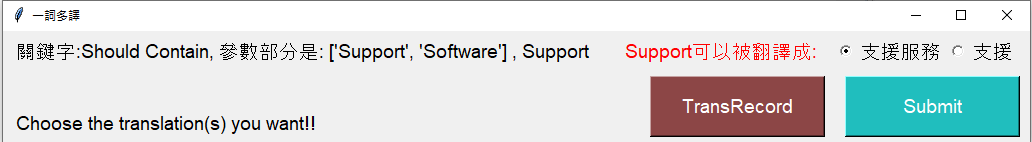
\includegraphics[width= 1.1\textwidth]{../論文截圖/3-4-1一詞多譯UI介面設計.png}
    \caption{一詞多譯UI的介面設計}
    \label{一詞多譯UI的介面設計}
\end{figure}

翻譯紀錄的介面設計(如圖~\ref{翻譯紀錄的介面設計}),本論文同樣將其設計成兩個區塊,上半部以條列式呈現設定檔中現存的使用者翻譯選擇。下半部包含一個Undo按鈕,考量到使用者可能不小心選錯了翻譯,用於將使用者的選擇從設定檔中刪除。
\begin{figure}[H]
    \centering
    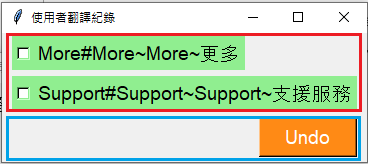
\includegraphics[width= .9\textwidth]{../論文截圖/3-4-2 翻譯紀錄介面設計.png}
    \caption{翻譯紀錄的介面設計}
    \label{翻譯紀錄的介面設計}
\end{figure}

一詞多譯UI的實作,大致可以分成8個部分: run()、draw\_trans\_options()、get\_transdic\_keys\_and\_values()、open\_record()、undo\_trans()、output\_setting\_file()、\\add\_trans\_info()、add\_keyword\_name()。各實作彼此之間的互動關係,則如圖~\ref{產生一詞多譯UI的sequence diagram}:
\hspace*{\fill} \\

\begin{figure}[H]
    \centering
    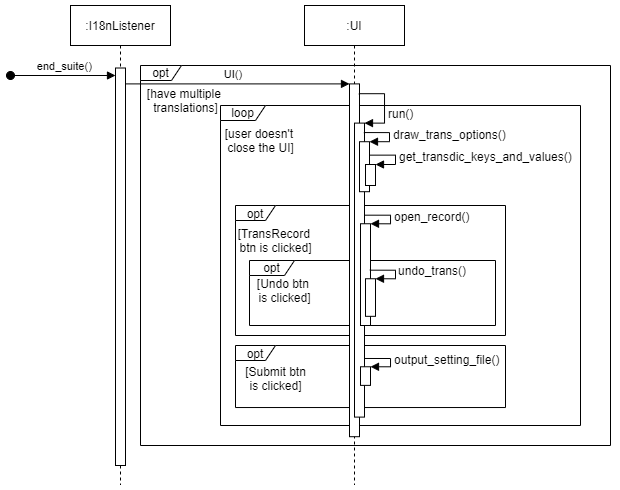
\includegraphics[width= \textwidth]{../UML/i18n sequence diagram-一詞多譯UI.png}
    \caption{產生一詞多譯UI的sequence diagram}
    \label{產生一詞多譯UI的sequence diagram}
\end{figure}

當測試腳本結束時,會呼叫I18nListener類別的end\_suite()函式。

若本次測試腳本遭遇一詞多譯,則呼叫UI類別,使其初始化並執行run()函式,產生一詞多譯UI的介面,包含“Choose the translation(s) you want!!” 字樣、顯示翻譯紀錄的 TransRecord按鈕,以及寫入使用者選擇的Submit按鈕。之後,run()函式內部會呼叫draw\_trans\_options()函式,其內會再呼叫get\_transdic\_keys\_and\_values()函式,取出待翻譯詞與其對應的翻譯,最後隨著翻譯當下的關鍵字名稱和參數部分一併顯示於一詞多譯UI的介面上。

在一詞多譯介面上,點擊TransRecord按鈕會呼叫open\_record()函式,打開翻譯紀錄介面,其會將先前使用者選擇過的翻譯詞,以條列式的方式呈現,且介面上還包含一顆Undo按鈕。點擊Undo按鈕會呼叫undo\_trans()函式,將使用者選擇的翻譯紀錄從設定檔中清除掉,同時關閉翻譯紀錄頁面。

在一詞多譯介面上,點擊Submit按鈕則會呼叫output\_setting\_file()函式,將使用者選擇的待翻譯詞對應其翻譯以及完整參數寫入設定檔“i18n/listeners/setting.txt”中,同時將剛剛已寫入的翻譯資訊從一詞多譯UI上隱藏。

此外,在UI類別中定義的add\_translations()和add\_keyword\_name()函式,雖然不會在一詞多譯UI執行期間被呼叫,但在測試腳本執行期間,卻能負責將代理關鍵字傳入的關鍵字名稱、待翻譯詞,與其對應翻譯,分別儲存於變數中,方便之後一詞多譯UI的讀取。並且,還會將關鍵字的參數部分和待翻譯詞結合,成為可以辨別「該次測試腳本是否執行過相同翻譯」的字串,存入unique\_log變數中。

\hspace*{\fill} \\
\\ \hspace*{\fill} \\

%3.5
\section{將i18n工具設計成為可以安裝的模組}
本論文透過Python的build模組,將i18n工具包裝成名為“RF-i18n-tool”的Library,並透過twine模組上傳至PYPI\cite{PYPI}網站上,使之成為可以直接讓使用者安裝的Python模組。解決了先前使用者只能從github上將i18n工具clone下來,並在該專案上開發測試腳本的不方便。

以下將詳述將i18n包裝成Python模組的步驟:

在將i18n工具打包成為一個Library前,必須先準備以下五個檔案: setup.cfg、pyproject.toml、README.md、LICENSE\cite{license}、MANIFEST.in。此外必須確認將打包的資料夾下,包含\_\_init\_\_.py檔案,以被系統辨識為一個Python模組。

上述的檔案準備就緒後,便可以在i18n專案目錄下執行python –m build 指令,待建置完畢,便會產生一個名為dist的資料夾,裡面裝著打包好的RF-i18n-tool模組檔案。接下來執行python –m twine upload - -repository pypi dist/* 指令,輸入帳號密碼後,便能成功將dist資料夾中的RF-i18n-tool模組上傳至PYPI了。之後在PYPI網站上搜尋RF-i18n-tool,便能看到上傳的模組。

使用者若要安裝此模組,只需執行pip install RF-i18n-tool 指令即可(如圖3.11)。

\begin{figure}[H]
    \centering
    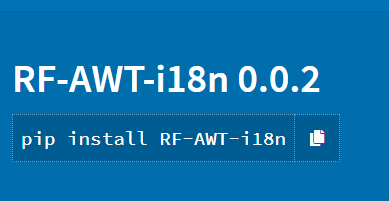
\includegraphics[width= .5\textwidth]{../論文截圖/3-5-8 安裝RF-AWT-i18n指令.png}
    \caption{安裝RF-i18n-tool指令}
\end{figure}

\hspace*{\fill} \\
\\ \hspace*{\fill} \\

最後,使用者便可透過在Additional Robot Framework arguments中設定系統參數(如圖~\ref{以i18n預設JSON翻譯檔來執行i18n工具}、~\ref{以使用者提供的JSON翻譯檔來執行i18n工具}),來使用i18n工具。自定義的JSON翻譯檔路徑必須遵守以下格式(如圖~\ref{JSON翻譯檔路徑格式})

\begin{figure}[H]
\begin{lstlisting}[language={python}]
-d out -L debug --listener %YOUR_PYTHON_PATH%/Lib/site-packages/i18n/listeners/I18nListener.py:YOUR_LOCALE:i18njson
\end{lstlisting}
\caption{以i18n預設JSON翻譯檔來執行i18n工具}
\label{以i18n預設JSON翻譯檔來執行i18n工具}
\end{figure}

\begin{figure}[H]
\begin{lstlisting}[language={python}]
-d out -L debug --listener %YOUR_PYTHON_PATH%/Lib/site-packages/i18n/listeners/I18nListener.py:YOUR_LOCALE
\end{lstlisting}
\caption{以使用者提供的JSON翻譯檔來執行i18n工具}
\label{以使用者提供的JSON翻譯檔來執行i18n工具}
\end{figure}

\begin{figure}[H]
\begin{lstlisting}[language={python}]
YOUR_PROJECT_DIR/languageFiles/YOUR_LOCALE(ex:zh-TW)/xxxYOUR_LOCALE.json
\end{lstlisting}
\caption{JSON翻譯檔路徑格式}
\label{JSON翻譯檔路徑格式}
\end{figure}
\chapter{測試案例分析}
本章節將為擴充的代理關鍵字撰寫單元測試\cite{ut},並且將改善翻譯邏輯與一詞多譯功能後的i18n工具,做功能的展示。最後將i18n工具套用至一個使用到多項代理關鍵字的Robot Framework測試腳本,以呈現“多國語言網頁自動化驗收測試”的效果。

%4.1
\section{新增與修改之代理關鍵字的單元測試}
以下將以Microsoft中文官方網頁\cite{microsoft},以及筆者使用Node.js\cite{nodejs}自行架設的i18n測試網頁(i18n Testing Website)為受測網站,為各個新增或已修改實作之代理關鍵字,分別提供Robot Framework的單元測試腳本,以驗證原生關鍵字在套用新的代理關鍵字下,能夠獨立正常運作。但為求精簡,本論文將不重複放上同類型關鍵字的測試腳本。(經修改的第一版i18n代理關鍵字前將加上‘*’標示)

%4.1.1
\subsection{Alert Should Be Present}
\begin{figure}[H]
\begin{lstlisting}[language={python}]
*** Settings ***
Library    SeleniumLibrary
Library    ../self_util.py
Test Setup    Run Keywords    Open Browser    http://localhost:3000    Chrome
...                    AND    Maximize Browser Window
Test Teardown    Close Browser

*** Test Cases ***
Alert should be present
    Wait until Element Is Visible    //*[normalize-space()='Show Alert Message']    timeout=${shortPeriodOfTime}
    Double Click Element    //*[normalize-space()='Show Alert Message']
    Alert Should Be Present    Welcome to Bing's website
\end{lstlisting}
\caption{Alert Should Be Present在代理關鍵字下執行的測試腳本}
\end{figure}
此測試腳本(如圖4.1)會打開i18n Testing Website,並雙擊Show Alert Message按鈕,使畫面跳出alert視窗(如圖4.2)。最後使用Alert Should Be Present來驗證alert資訊是否為“歡迎光臨Bing的網頁”。測試通過,代表參數“Welcome to Bing’s website”有成功被翻譯為“歡迎光臨Bing的網頁”(如圖4.3)。

\begin{figure}[H]
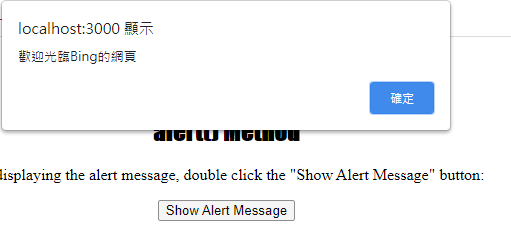
\includegraphics[width= \textwidth]{../論文截圖/4-1-2 alert視窗的文字.png}
\caption{網頁上的alert視窗顯示的文字}
\end{figure}

\begin{figure}[H]
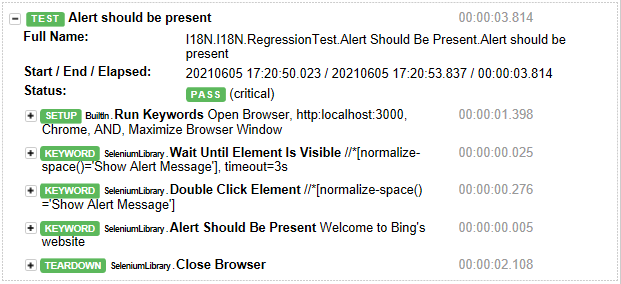
\includegraphics[width= \textwidth]{../論文截圖/4.1.1-3 pass.png}
\caption{Alert Should Be Equal測試通過}
\end{figure}

\hspace*{\fill} \\
\\ \hspace*{\fill} \\
\\ \hspace*{\fill} \\
\\ \hspace*{\fill} \\
\\ \hspace*{\fill} \\
%4.1.2
\subsection{Count Values In List}
\begin{figure}[H]
\begin{lstlisting}[language={python}]
*** Test Cases ***
Count values in list
    @{list1} =    Create List    支援    Software
    ${number} =    Count Values In List    ${list1}    Support
    Log    ${number}
\end{lstlisting}
\caption{Count Values In List在代理關鍵字下執行的測試腳本}
\end{figure}
此測試腳本(如圖4.4),一開始會利用Create List創出一個包含「支援」和‘Software’的list,並使用Count Values In List來計算參數‘Support’出現在此list中幾次。第一次執行測試通過(如圖4.5),透過Log印出的數字為1,代表參數‘Support’被翻譯為「支援」後,出現在list中一次,所以測試通過;且系統將支援當成“Support”翻譯的其中一種,並跳出一詞多譯UI。之後,使用者選擇「支援」作為唯一翻譯。第二次測試通過(如圖4.6),透過Log印出的數字為1,且不跳出一詞多譯UI與warning資訊。

\begin{figure}[H]
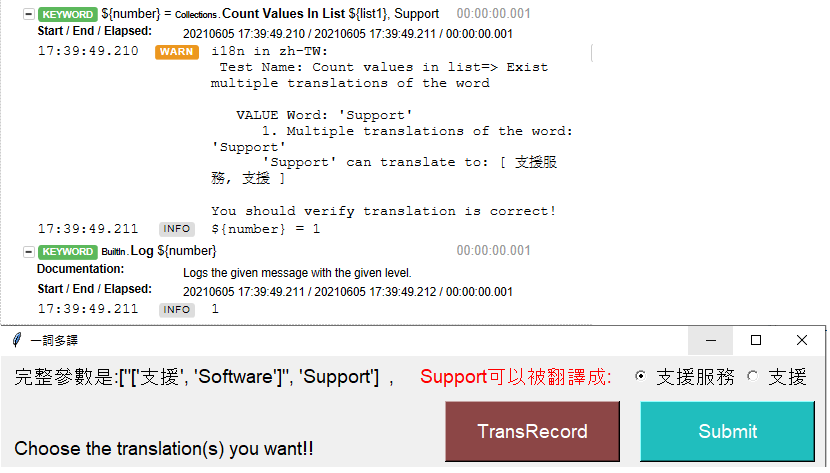
\includegraphics[width= \textwidth]{../論文截圖/4.1.2-2 count values in list 1st run.png}
\caption{Count Values In List測試腳本第一次執行通過}
\end{figure}

\begin{figure}[H]
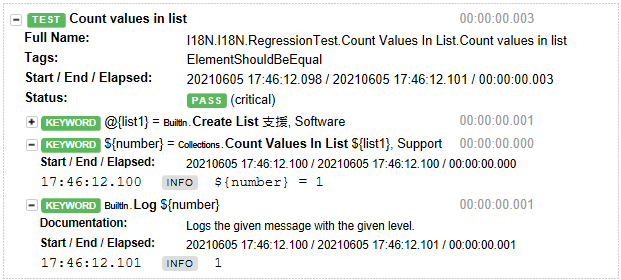
\includegraphics[width= \textwidth]{../論文截圖/4.1.2-3 count values in list 2nd run.png}
\caption{Count Values In List測試腳本第二次執行通過}
\end{figure}

\hspace*{\fill} \\
\\ \hspace*{\fill} \\
\\ \hspace*{\fill} \\
\\ \hspace*{\fill} \\
\\ \hspace*{\fill} \\
%4.1.3
\subsection{Dictionaries Should Be Equal}
\begin{figure}[H]
\begin{lstlisting}[language={python}]
*** Test Cases ***
Dictionaries should be equal
&{dict1} =    Create Dictionary    軟體=支援
&{dict2} =    Create Dictionary    Software=Support
Dictionaries Should Be Equal    ${dict1}    ${dict2}
\end{lstlisting}
\caption{Dictionaries Should Be Equal在代理關鍵字下執行的測試腳本}
\end{figure}
此測試腳本(如圖4.7),會利用Create Dictionary創出兩個dictionaries,分別是{'軟體': '支援'}和{'Software', 'Support'}(測試腳本的 ‘=’左側為key,右側為value),並使用Dictionaries Should Be Equal檢查兩者是否相同。第一次執行測試通過(如圖4.8),代表dictionary {‘Software’, ‘Support’}有成功被翻譯,且系統將“支援”當成“Support”翻譯的其中一種,並跳出一詞多譯UI。之後,使用者選擇“支援”作為唯一翻譯。第二次測試通過(如圖4.9),且不跳出一詞多譯UI與warning資訊,代表’Support’ 根據使用者選擇成功被翻譯為‘支援’。

\begin{figure}[H]
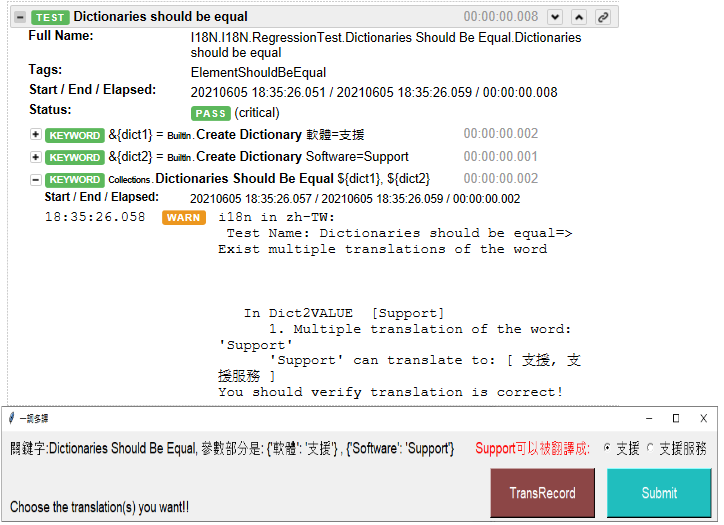
\includegraphics[width= \textwidth]{../論文截圖/4.1.3-2 dictionaries should be equal 1st run.png}
\caption{Dictionaries Should Be Equal測試腳本第一次執行通過}
\end{figure}

\begin{figure}[H]
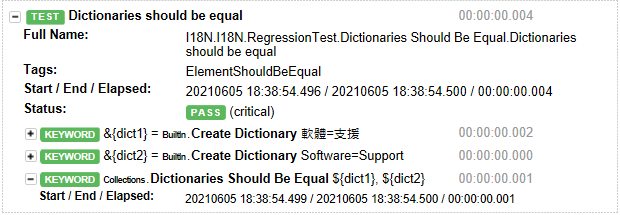
\includegraphics[width= \textwidth]{../論文截圖/4.1.3-3 dictionaries should be equal 2nd run.png}
\caption{Dictionaries Should Be Equal測試腳本第二次執行通過}
\end{figure}

%4.1.4
\subsection{Select From List By Label}
\begin{figure}[H]
\begin{lstlisting}[language={python}]
*** Settings ***
Resource    ../CommonVariables.txt
Library    SeleniumLibrary
Test Setup    Run Keywords    Open Browser    http://localhost:3000    Chrome
...                    AND    Maximize Browser Window
Test Teardown    Close Browser

*** Test Cases ***
Select from list by the label "Support"
${defaultSelection} =    Set Variable    //*[@id='i18n-selection-list']//*[text()='Software' and @selected]
${selectionList} =    Set Variable    //*[@id='i18n-selection-list']
Wait Until Element Is Visible    ${defaultSelection}    timeout=${shortPeriodOfTime}
Select From List By Label    ${selectionList}    Support
List Selection Should Be    ${selectionList}    Support
\end{lstlisting}
\caption{Select From List By Label在代理關鍵字下執行的測試腳本}
\end{figure}
此測試腳本(如圖4.10),會打開i18n Testing Website,並使用Select From List By Label選取畫面上selection list的Support選項(如圖4.11)。之後用List Selection Should Be驗證結果是否正確。第一次測試通過(如圖4.12),而畫面上選擇了‘支援’,代表參數Support有成功被翻譯,且系統將‘支援’當作‘Support’的其中一種翻譯,隨後跳出了一詞多譯UI。之後,使用者選擇了‘支援服務’當作Support的唯一翻譯。第二次測試腳本通過(如圖4.13),畫面上被選擇的selection list顯示‘支援服務’,代表參數‘Support’成功被翻譯為使用者前一次的選擇。

\begin{figure}[H]
\centering
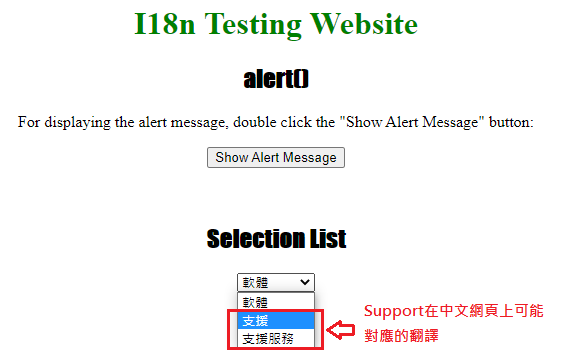
\includegraphics[width= .6\textwidth]{../論文截圖/4-1-7 Select from list by label要驗證的網頁元件.png}
\caption{Select From List By Label測試腳本要驗證的網頁元件}
\end{figure}

\begin{figure}[H]
\centering
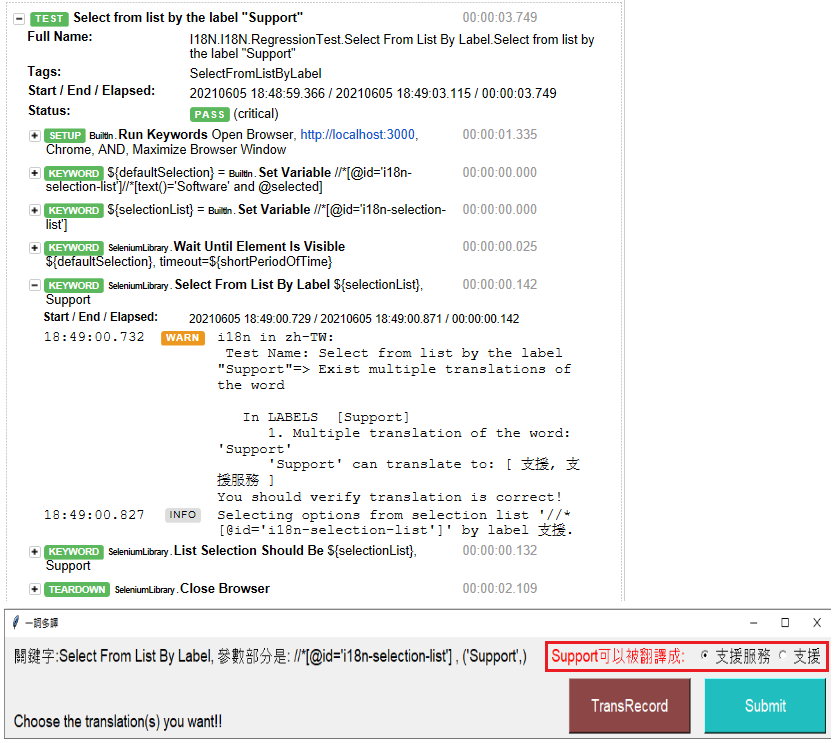
\includegraphics[width= .8\textwidth]{../論文截圖/4.1.4-2 select from list by label 1st run.png}
\caption{Select From List By Label測試腳本第一次執行通過}
\end{figure}

\begin{figure}[H]
\centering
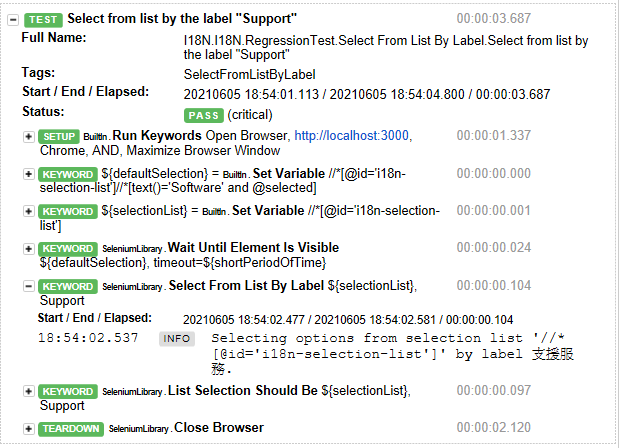
\includegraphics[width= .8\textwidth]{../論文截圖/4.1.4-3 select from list by label 2nd run.png}
\caption{Select From List By Label測試腳本第二次執行通過}
\end{figure}

\hspace*{\fill} \\
\\ \hspace*{\fill} \\
\\ \hspace*{\fill} \\
\\ \hspace*{\fill} \\
\\ \hspace*{\fill} \\
%4.1.5
\subsection{*Page Should Contain Element}
\begin{figure}[H]
\begin{lstlisting}[language={python}]
*** Settings ***
Resource    ../CommonVariables.txt
Library    SeleniumLibrary
Library    ../self_util.py
Test Setup    Run Keywords    Open Browser To Microsoft Page
...                    AND    Change Language    expectedLanguage=${language}
Test Teardown    Close Browser

*** Test Cases ***
Check "Microsoft Support" webelement is on the support page
    Go To Support Page
    ${MicrosoftSupport} =    Set Variable    //*[@id ='supHomeAndLandingPageHeaderContainer']//*[contains(text(), 'Support')]
    Page Should Contain Element    ${MicrosoftSupport}
\end{lstlisting}
\caption{*Page Should Contain Element在代理關鍵字下執行的測試腳本}
\end{figure}
此測試腳本(如圖4.14),會打開Microsoft中文官方網頁,前往支援頁面,之後使用Page Should Contain Element驗證畫面上的Support文字(如圖4.15)。第一次測試通過(如圖4.16),代表參數Support有成功被翻譯,且系統將‘支援服務’當作‘Support’的其中一種翻譯,隨後跳出了一詞多譯UI。之後,使用者選擇了‘支援服務’當作Support的唯一翻譯。第二次測試腳本通過(如圖4.17),且沒有跳出一詞多譯UI,代表參數‘Support’成功被翻譯為使用者前一次的選擇。

\begin{figure}[H]
\centering

\includegraphics[width= .8\textwidth]{../論文截圖/4-1-9 Page should contain element要驗證的網頁元件.png}
\caption{*Page Should Contain Element 測試腳本要驗證的網頁元件}
\end{figure}

\begin{figure}[H]
\centering
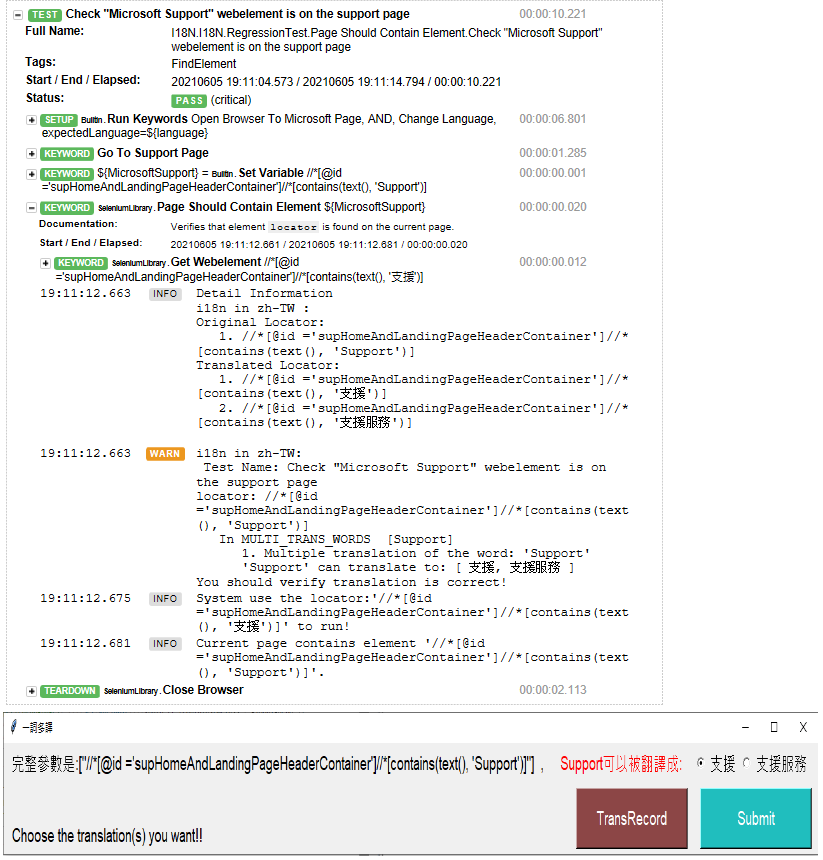
\includegraphics[width= .8\textwidth]{../論文截圖/4.1.5-2 page should contain element 1st run.png}
\caption{*Page Should Contain Element測試腳本第一次執行通過}
\end{figure}
\begin{figure}[H]
\centering
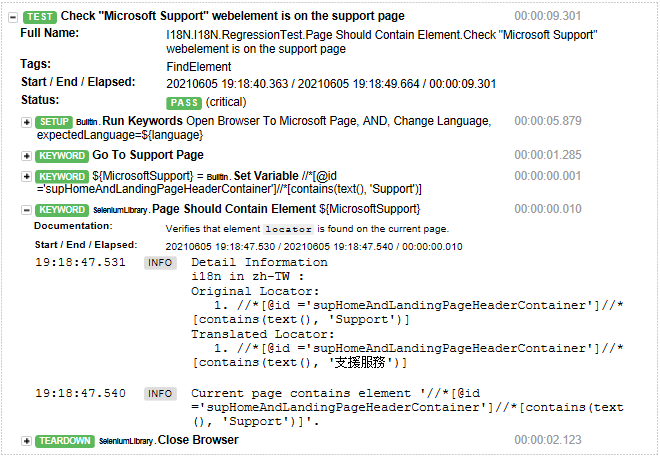
\includegraphics[width= \textwidth]{../論文截圖/4.1.5-3 page should contain element 2nd run.png}
\caption{*Page Should Contain Element測試腳本第二次執行通過}
\end{figure}

\hspace*{\fill} \\
\\ \hspace*{\fill} \\
\\ \hspace*{\fill} \\
\\ \hspace*{\fill} \\
\\ \hspace*{\fill} \\
%4.1.6
\subsection{Table Should Contain}
\begin{figure}[H]
\begin{lstlisting}[language={python}]
*** Settings ***
Resource    ../CommonVariables.txt
Library    SeleniumLibrary
Library    ../self_util.py
Test Setup    Run Keywords    Open Browser    http://localhost:3000    Chrome
...                    AND    Maximize Browser Window
Test Teardown    Close Browser

*** Test Cases ***
Table should contain "Support"
    ${table} =    Set Variable    //*[@id='i18n-table']
    Wait Until Element Is Visible    ${table}    timeout=${shortPeriodOfTime}
    Table Should Contain    ${table}    Support
\end{lstlisting}
\caption{Table Should Contain在代理關鍵字下執行的測試腳本}
\end{figure}
此測試腳本(如圖4.18),會打開I18n Testing Website,之後使用Table Should Contain 驗證畫面上的Support文字(如圖4.19)。第一次測試通過(如圖4.20),代表參數‘Support’有成功被翻譯,且系統將‘支援’當作‘Support’的其中一種翻譯,隨後跳出了一詞多譯UI。之後,使用者選擇了‘支援’當作‘Support’的唯一翻譯。第二次執行測試腳本通過(如圖4.21),且沒有跳出一詞多譯UI,代表參數‘Support’成功被翻譯為使用者前一次的選擇。

\begin{figure}[H]
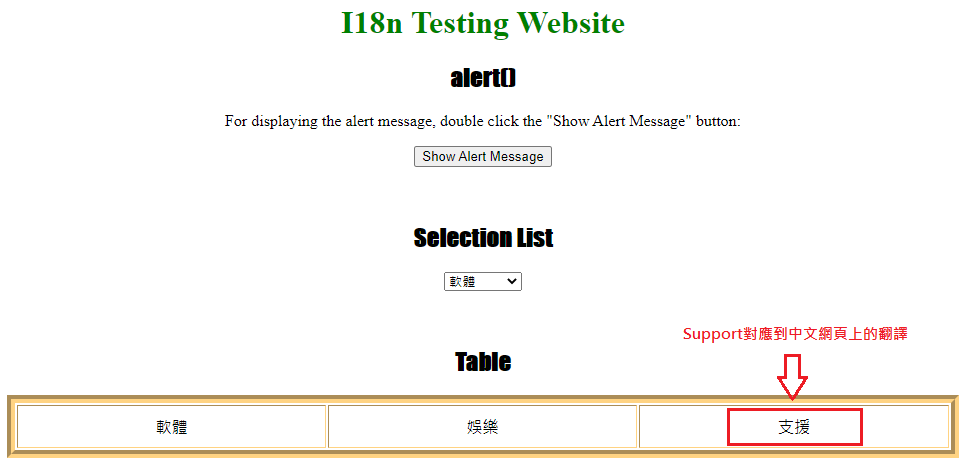
\includegraphics[width= \textwidth]{../論文截圖/4-1-13 Table should contain要驗證的網頁元件.png}
\caption{Table Should Contain 測試腳本要驗證的網頁元件}
\end{figure}

\begin{figure}[H]
\includegraphics[width= \textwidth]{../論文截圖/4.1.6-2 table should contain 1st run.png}
\caption{Table Should Contain 測試腳本第一次執行通過}
\end{figure}

\begin{figure}[H]
\includegraphics[width= \textwidth]{../論文截圖/4.1.6-3 table should contain 2nd run.png}
\caption{Table Should Contain 測試腳本第二次執行通過}
\end{figure}

\hspace*{\fill} \\
\\ \hspace*{\fill} \\
\\ \hspace*{\fill} \\
\\ \hspace*{\fill} \\
\\ \hspace*{\fill} \\
%4-2
\section{改善翻譯邏輯後的驗收測試示例}
以下將舉Page Should Contain Element關鍵字的測試腳本為例,去驗證Microsoft中文官方網頁上的文字。並說明在改善XPath翻譯邏輯前後,執行含有@placeholder屬性的XPath之腳本,將分別得到何種結果。

\begin{figure}[H]
\begin{lstlisting}[language={python}]
*** Settings ***
Resource    ../CommonVariables.txt
Library    SeleniumLibrary
Library    ../self_util.py
Test Setup    Run Keywords    Open Browser To Microsoft Page
...                    AND    Change Language    expectedLanguage=${language}
Test Teardown    Close Browser

*** Test Cases ***
Test web element is on the support page by given special attributes
    Go To Support Page
    ${MicrosoftSupport} =    Set Variable    //*[@id ='supHomeAndLandingPageSearchBox' and @placeholder ='How can we help you?']
    Page Should Contain Element    ${MicrosoftSupport}
\end{lstlisting}
\caption{含有@placeholder屬性的XPath之測試腳本}
\end{figure}

\begin{figure}[H]
\centering

\includegraphics[width= .9\textwidth]{../論文截圖/4-2-2 畫面上@placeholder的實際文字.png}
\caption{中文版Microsoft網頁@placeholder屬性對應的實際文字\cite{microsoft}}
\end{figure}

\begin{figure}[H]
\centering
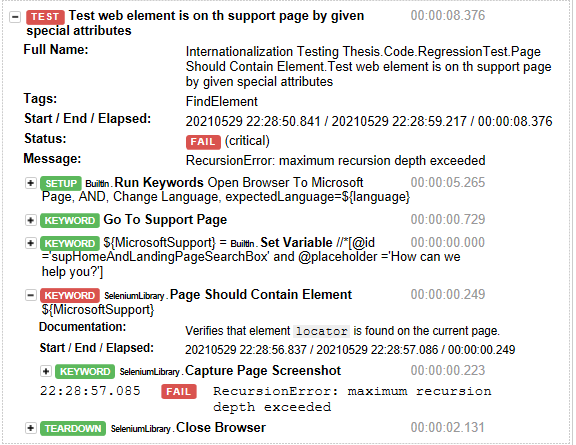
\includegraphics[width= .8\textwidth]{../論文截圖/4-2-3 @placeholder運行在第一版i18n.png}
\caption{待翻譯XPath運行在未改善翻譯邏輯時的i18n工具之結果}
\end{figure}

\begin{figure}[H]
\centering
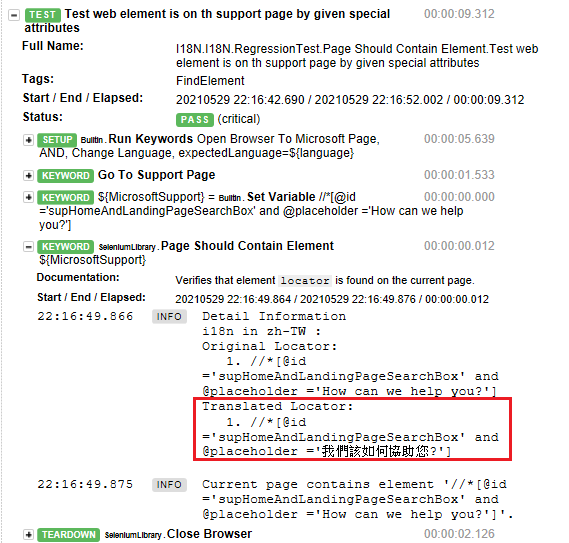
\includegraphics[width= \textwidth]{../論文截圖/4-2-4 @placeholder運行在當前i18n版本.png}
\caption{待翻譯XPath運行在改善翻譯邏輯後的i18n工具之結果}
\end{figure}

由以上的結果我們可以發現,第一版的i18n工具,會因為無法對XPath內的@placeholder屬性做翻譯,而使得測試發生錯誤。本論文新版的i18n工具,因為改善了翻譯邏輯,所以支援各種HTML屬性的翻譯。並成功將”how can we help you?”翻譯為”我們該如何協助您”,進而使測試通過。

%4-3
\section{一詞多譯情況下所產生的圖形化使用者介面}
在遭遇一詞多譯且測試腳本會通過的情況下,以Test should be equal為例(如圖4.26);分別創出兩個變數word1、word2,並用Should Be Equal檢驗兩個變數的值是否正確。測試執行結束後,系統會產生一個圖形化使用者介面(如4.27),上面分別記錄了遭遇一詞多譯的關鍵字完整參數,以及所有可能的翻譯詞,供使用者做選擇。\\

\begin{figure}[H]
\begin{lstlisting}[language={python}]
*** Settings ***
Test should be equal
    ${word1} =    Set Variable    More
    ${word2} =    Set Variable    Support
    Should Be Equal    ${word1}    More
    Should Be Equal    ${word2}    Support
\end{lstlisting}
\caption{Test should be equal 測試腳本}
\end{figure}

\begin{figure}[H]
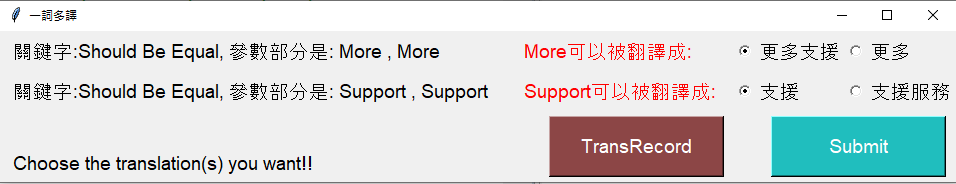
\includegraphics[width= \textwidth]{../論文截圖/4-3-2 測試通過且有一詞多譯時,UI會跳出.png}
\caption{遭遇一詞多譯且測試通過,開啟一詞多譯UI}
\end{figure}

當使用者選擇了希望的翻譯並按下Submit按鈕後,系統便會產生一份設定檔,以利下次執行到同一份腳本的同一關鍵字時,直接套用選擇的翻譯,同時清空一詞多譯介面上的翻譯選項(如圖4.28)。

\begin{figure}[H]
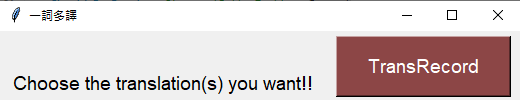
\includegraphics[width= \textwidth]{../論文截圖/4-3-3 選擇翻譯後,清空選項.png}
\caption{按下Submit按鈕後,將翻譯寫進設定檔,同時清除翻譯選項}
\end{figure}

假如使用者選擇錯誤時,則可以點擊TransRecord按鈕來打開翻譯紀錄的介面,上面記錄著使用者曾經的翻譯選擇,並有一顆Undo按鈕(如圖4.29)。使用者選擇了要清除的翻譯紀錄後,按下Undo按鈕,系統便會將設定檔中的該資料刪除,同時關閉翻譯紀錄介面,當再次打開翻譯紀錄介面時,可以發現被選擇清除的資料已消失(如圖4.30)。

\begin{figure}[H]
\centering
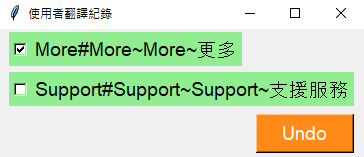
\includegraphics[width= .5\textwidth]{../論文截圖/4-3-4 介面上記錄著使用者翻譯選擇.png}
\caption{打開翻譯紀錄介面,上面記錄著使用者翻譯選擇}
\end{figure}

\begin{figure}[H]
\centering

\includegraphics[width= .5\textwidth]{../論文截圖/4-3-5 將選擇的翻譯清除後,再次打開翻譯紀錄介面.png}
\caption{清除選擇的翻譯紀錄後,再次打開翻譯紀錄介面}
\end{figure}

然而,並非所有的測試腳本都會遭遇一詞多譯,且總是通過。因此,底下將分別說明在其他兩種情況下,系統會有甚麼不同的反應:

\begin{itemize}
\item[1.]測試腳本不通過:
若測試腳本不通過,則不論遭遇一詞多譯與否,皆不會跳出一詞多譯UI。其設計想法為,因為系統有檢驗的機制,所以此刻測試腳本不會通過,則代表原先未翻譯前的測試腳本也不會通過。而為原先就會發生錯誤的待翻譯詞選擇其翻譯,對使用者而言,顯然是毫無意義的,但是為了測試結果的完整性,系統還是會於測試報表上顯示一詞多譯的warning資訊(如圖4.31)。
\begin{figure}[H]
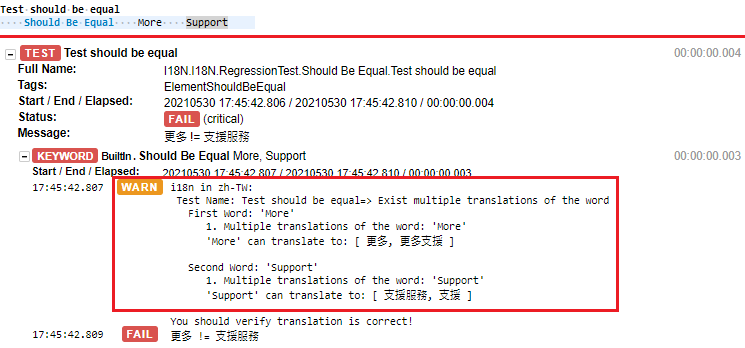
\includegraphics[width= \textwidth]{../論文截圖/4-3-6 測試腳本fail,不跳UI.png}
\caption{測試腳本不通過的情況下,不跳出UI,但會顯示warning資訊於報表}
\end{figure}
\item[2.]測試腳本通過,且沒有遭遇一詞多譯: 
在測試腳本通過且沒有遭遇一詞多譯的情況下,測試結束後便不會跳出一詞多譯UI介面。但有一種情況是,關鍵字的參數部分原本會遭遇一詞多譯,但因為前一次執行時使用者已針對此待翻譯詞選擇了翻譯,所以被系統視為只有一種翻譯,因此不跳出一詞多譯UI(如圖4.32)。(有關系統如何判定翻譯已被使用者選擇,詳見本論文3-2節)
\begin{figure}[H]
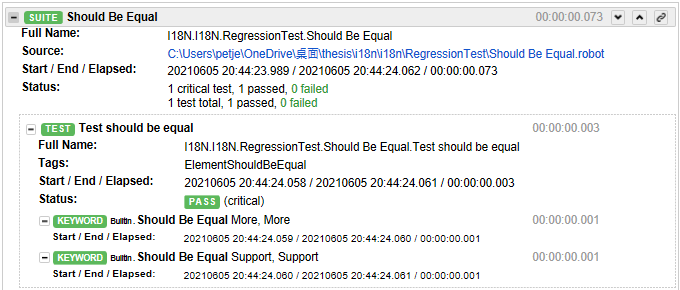
\includegraphics[width= \textwidth]{../論文截圖/4-3-7 測試腳本pass且沒一詞多譯,不跳UI.png}
\caption{測試腳本通過且沒有遭遇一詞多譯的情況下,不跳出UI}
\end{figure}
\end{itemize}

%4-4
\section{使用涵蓋多項代理關鍵字的測試腳本}
以上介紹的測試案例,分別呈現了本論文各項功能改善後的實際成果,但因為都偏向單一關鍵字或單一功能的測試,在此將設計一個較複雜的Robot Framework網頁自動化驗收測試腳本,內部使用到多種代理關鍵字,來對Microsoft的中文版網頁進行一系列操作。同時,會遭遇到一詞多譯,並且會使用相別於第一版i18n所列舉的html待翻譯屬性來撰寫XPath。藉此來對新版i18n工具作一個驗收測試。

以下將執行Test multiple user behaviors on Microsoft website測試腳本兩次,分別呈現選擇一詞多譯翻譯前後,測試結果有何差異之處。

\begin{figure}[H]
\begin{lstlisting}[language={python}]
*** Settings ***
Resource    ./Keywords.txt
Library    SeleniumLibrary
Test Setup    Run Keywords    Open Browser To Microsoft Page
...                    AND    Change Language    expectedLanguage=${language}
Test Teardown    Close Browser

*** Test Cases ***
Test multiple user behaviors on Microsoft website
    Go To Support Page
    Support Button Text Should Be    Support
    Wait Until Element Is Visible    //*[@id = 'uhfCatLogo' ]//*[normalize-space()='Support']
    Click Element    //*[@id = 'uhfCatLogo' ]//*[normalize-space()='Support']
    ${MicrosoftSupport} =    Set Variable    //*[@id ='supHomeAndLandingPageHeaderContainer']//*[contains(text(), 'Support')]
    Page Should Contain Element    ${MicrosoftSupport}

*** Keywords ***
Support Button Text Should Be
    [Arguments]    ${expected}
    ${supportButton} =    Set Variable    //*[@id ='uhfCatLogo']
    Element Text Should Be    ${supportButton}    ${expected}
\end{lstlisting}
\caption{Test multiple user behaviors on Microsoft website測試腳本實作}
\end{figure}
此測試腳本(如圖4.33),會打開Microsoft中文官方網頁,先到支援頁面,之後點擊‘支援’的Logo,到新的支援頁面。最後,驗證畫面上的橫向標語有包含‘支援服務’字樣。因為同時遭遇到3種Support需要被翻譯,系統便會逐一將它們紀錄下來,待測試腳本結束後,分別顯示於一詞多譯UI上。

\begin{figure}[H]
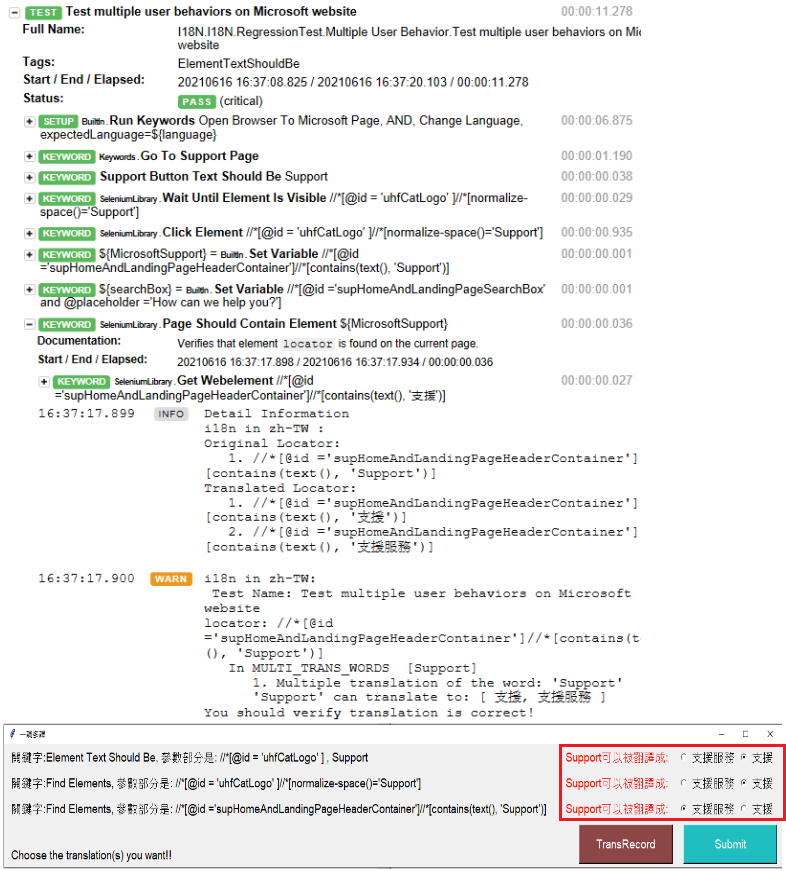
\includegraphics[width= \textwidth]{../論文截圖/4-4-2 test multiple user behaviors測試腳本1st run.png}
\caption{Test multiple user behaviors on Microsoft website測試腳本第一次執行結果}
\end{figure}

第一次執行測試腳本(如圖4.34)結束後,使用者分別為三種不同情況下遭遇一詞多譯的Support,選擇了支援、支援、支援服務為其正確翻譯,並點擊Submit按鈕,將選擇寫入設定檔中。

\begin{figure}[H]
\centering
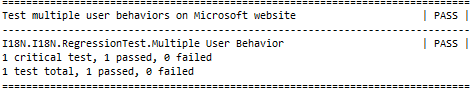
\includegraphics[width= .9\textwidth]{../論文截圖/4-4-3 test multiple user behaviors測試腳本2nd run.png}
\caption{Test multiple user behaviors on Microsoft website測試腳本第二次執行結果}
\end{figure}

第二次執行測試腳本時(如圖4.35),會根據設定檔內的翻譯紀錄,分別對三種Support進行翻譯。因為被系統判定為單一翻譯,所以測試結束後,並不會顯示一詞多譯UI。

\chapter{結論與未來展望}

%5.1
\section{結論}
本論文提出了四項措施去改進第一版i18n工具所面臨的問題,分別是擴充代理關鍵字、支援所有HTML屬性的XPath翻譯邏輯、支援自由選擇翻譯的一詞多譯圖形化使用者介面、可以提供安裝的Python模組。透過以上努力,即可讓使用此i18n工具的多國語言網頁自動化驗收測試腳本,不再侷限於只能使用特定的關鍵字去撰寫。並且XPath的撰寫也不再需要考慮只有@title、text()、normalize-space()會被翻譯的問題,使用者的測試腳本可以用更多元的XPath寫法來搭配此i18n工具使用。遭遇一詞多譯時,使用者也能夠在第一次測試腳本結束後,選擇內心所預期的翻譯詞來執行接下來的測試。最後,藉由將i18n工具包裝成可以pip install 的Python模組,使用者可以隨安裝即使用本工具所提供的功能,而無須將自己的測試腳本移動到i18n工具的資料夾下。

\hspace*{\fill} \\
\\ \hspace*{\fill} \\
\\ \hspace*{\fill} \\
%5.2
\section{i18n工具的使用限制與未來展望}
本論文的i18n工具尚存在著使用限制,其原因之一源自於某些Robot Framework的原生關鍵字,其參數部分接受的是特殊的字元,目前i18n工具是不支援的。如圖5.1,Get Match Count接受的第二個參數是‘S*’,用來抓出串列中符合的字串,若是強行將‘S*’翻譯,便會直接導致測試結果出錯。

\begin{figure}[H]
\centering
\begin{lstlisting}[language={python}]
*** Test Cases ***
Get match count
    @{list1} =    Create List   Support    Software    Apple
    ${count} =    Get Match Count    ${list1}    S*
    Log    ${count} 
\end{lstlisting}
\caption{Get Match Count測試腳本}
\end{figure}

此外,某些Robot Framework的關鍵字,其內部實作會呼叫另一個原生的關鍵字,且被呼叫的關鍵字也有一詞多譯的需求。當使用者為第一次執行測試的一詞多譯選擇了翻譯後,並執行第二次測試腳本時,因為此時傳入代理關鍵字的參數部分已改變,系統會將其判定為不同的待翻譯詞,而需要使用者事後再選擇一次。如圖5.2 ,Dictionary Should Contain Item原生關鍵字的實作會呼叫Dictionary Should Contain Key(如圖5.3紅色框起部分),導致第一次執行測試時傳入的‘More’,和第二次執行時傳入的‘More’,由於參數紀錄的局部從[‘支援’,‘支援服務’]變成[‘支援’],因此被系統判定成不同的待翻譯詞,需要重新選擇(如圖5.4)。\\

\begin{figure}[H]
\centering
\begin{lstlisting}[language={python}]
*** Test Cases ***
Dictionary should contain item
    &{dict1} =    Create Dictionary    More=Support
    Dictionary Should Contain Item    ${dict1}    More    Support
\end{lstlisting}
\caption{Dictioanry Should Contain Item測試腳本}
\end{figure}

\begin{figure}[H]
\centering
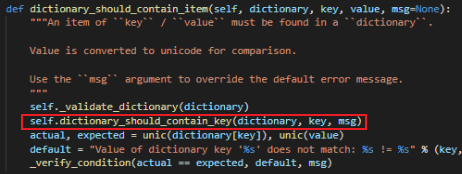
\includegraphics[width= \textwidth]{../論文截圖/5-1-2 dictionary should contain item測試腳本與其原生實作.png}
\caption{Dictioanry Should Contain Item原生實作}
\end{figure}

\begin{figure}[H]
\centering
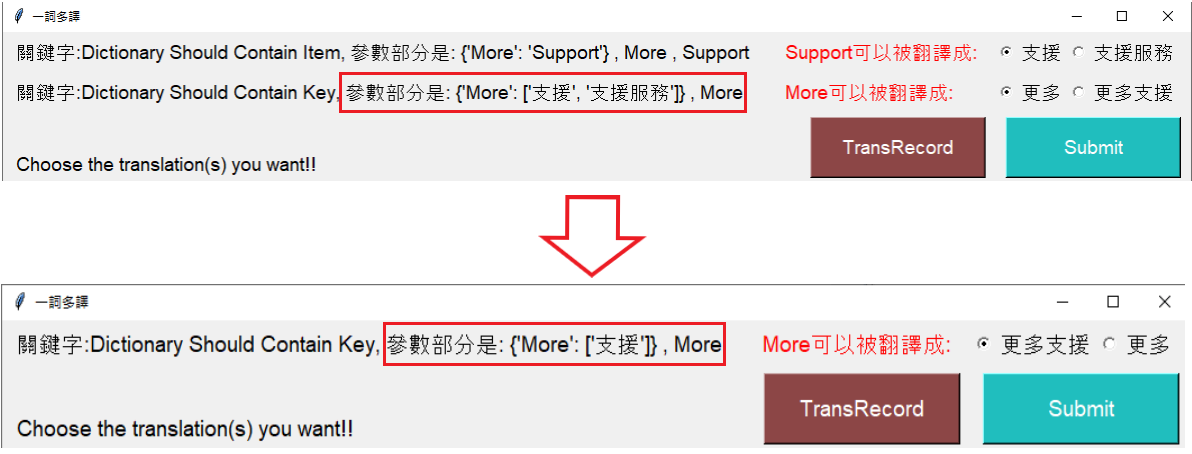
\includegraphics[width= \textwidth]{../論文截圖/5-1-3 1st&2nd執行測試腳本,待翻譯詞的參數紀錄變化.png}
\caption{第一次與第二次執行測試腳本,待翻譯詞的參數紀錄變化}
\end{figure}

未來展望的部分,可以根據i18n工具尚存在的使用限制,未來朝向優化特殊字元的翻譯方式,以及改善重複翻譯詞的判定邏輯去努力。而且目前JSON翻譯檔還需要由使用者提供,未來可以研究如何透過設計爬蟲,抓取多國語言網頁上的對應翻譯詞,自動將JSON翻譯檔產生出來,將人工的成本降低。進而讓「多國語言網頁自動化驗收測試」工具變得更貼近測試者的需要,錯誤率低且容易使用。

\vfill
\newpage
\addcontentsline{toc}{chapter}{參考文獻}

\bibliographystyle{unsrt}
\bibliography{reference}


\end{document}
